\documentclass[10pt]{article}

\usepackage[letterpaper,margin=0.82in]{geometry}
\usepackage{times}
\usepackage{microtype}
\usepackage{amsmath}
\usepackage{amssymb}
\usepackage{booktabs}
\usepackage{array}
\usepackage{enumitem}
\usepackage{tabularx}
\usepackage{longtable}
\usepackage{listings}
\usepackage{needspace}
\usepackage{float}
\usepackage{xcolor}
\usepackage{xspace}
\usepackage{tikz}
\usetikzlibrary{arrows.meta,fit,positioning,calc}
\usepackage[hidelinks]{hyperref}
\usepackage{fancyhdr}

\definecolor{amosblue}{HTML}{173B57}
\definecolor{amoslight}{HTML}{EEF4F7}
\definecolor{amosgreen}{HTML}{EAF4EF}
\definecolor{amosorange}{HTML}{FAF1E5}
\definecolor{amosgray}{HTML}{F3F4F5}

\hypersetup{
  pdftitle={AMOS: A Memory Operating Layer for Autonomous Data Analysis},
  pdfauthor={Elton Chang},
  pdfsubject={End-to-end AMOS product architecture and implementation guide}
}

\pagestyle{fancy}
\fancyhf{}
\fancyhead[L]{\small\textcolor{amosblue}{AMOS Product Architecture}}
\fancyhead[R]{\small\textcolor{gray}{End-to-End Build Guide}}
\fancyfoot[C]{\small\thepage}
\renewcommand{\headrulewidth}{0.3pt}
\setlength{\headheight}{14pt}

\setlength{\parindent}{0pt}
\setlength{\parskip}{0.38em}
\setlist[itemize]{leftmargin=1.22em,itemsep=0.12em,topsep=0.18em}
\setlist[enumerate]{leftmargin=1.42em,itemsep=0.14em,topsep=0.18em}
\renewcommand{\arraystretch}{1.11}
\newcolumntype{L}[1]{>{\raggedright\arraybackslash}p{#1}}
\newcolumntype{C}[1]{>{\centering\arraybackslash}p{#1}}
\newcolumntype{Y}{>{\raggedright\arraybackslash}X}
\newcommand{\amos}{\textsc{AMOS}\xspace}
\newcommand{\code}[1]{\texttt{#1}}
\newcommand{\idcode}[1]{\nolinkurl{#1}}
\newcommand{\atxn}{\textsc{A-TXN}\xspace}
\newcommand{\must}{\textbf{\textcolor{amosblue}{MUST:}}\xspace}
\newcommand{\should}{\textbf{\textcolor{amosblue}{SHOULD:}}\xspace}
\newcommand{\may}{\textbf{\textcolor{amosblue}{MAY:}}\xspace}
\newcommand{\deferred}{\textbf{\textcolor{gray}{DEFERRED:}}\xspace}
\newcommand{\nongoal}{\textbf{\textcolor{gray}{NON-GOAL:}}\xspace}
\newcommand{\mem}{\mathcal{M}}
\newcommand{\state}{\mathcal{S}}
\newcommand{\work}{\mathcal{W}}
\newcommand{\prov}{\mathcal{G}}
\lstdefinestyle{contract}{
  basicstyle=\ttfamily\scriptsize,
  breaklines=true,
  columns=fullflexible,
  frame=single,
  rulecolor=\color{gray!45},
  backgroundcolor=\color{amosgray},
  showstringspaces=false,
  keepspaces=true,
  aboveskip=0.45em,
  belowskip=0.45em
}
\BeforeBeginEnvironment{lstlisting}{\Needspace{0.48\textheight}}
\tikzset{
  seqactor/.style={draw=amosblue,rounded corners=1.5pt,fill=amoslight,font=\scriptsize,minimum height=5mm,align=center},
  seqlife/.style={draw=gray!65,dashed,thin},
  seqmsg/.style={-Latex,draw=amosblue,thin},
  seqfail/.style={-Latex,draw=red!65!black,thin},
  seqnote/.style={font=\scriptsize,fill=amosorange,draw=orange!65!black,rounded corners=1pt,inner sep=2pt,align=center}
}

\begin{document}

\begin{center}
  {\fontsize{20}{23}\selectfont\bfseries\textcolor{amosblue}{AMOS: A Memory Operating Layer\\for Autonomous Data Analysis}}
\end{center}

\begin{abstract}
This document is the product architecture and build guide for \amos. It defines the theory, system boundaries, data model, runtime protocol, component interfaces, security model, deployment topology, operating model, and phased implementation plan needed to build \amos from an empty repository to a production service. The intended reader is a startup engineering team that must make the system work, operate it safely, and know when each layer is complete.

\amos is a model-neutral operating layer between autonomous data-analysis applications and a company's data systems. It converts changing schemas, metrics, snapshots, documents, permissions, prior analyses, reviewer corrections, and execution records into governed analytical memory. For each task, it compiles a bounded working set, grants scoped tool capabilities, validates the versions used, verifies the computation, records claim-level support, and commits the artifact with a replay and invalidation contract. Models propose plans and interpretations; deterministic services retain authority over access, execution, validation, and publication.

The architecture is deliberately incremental. A startup first ships a modular monolith that completes one read-only analytical workflow end to end. It then adds durable feedback, scheduling, multi-tenant governance, connector breadth, and controlled autonomy only after explicit correctness, security, reliability, and customer-value gates pass. The guide defines the complete subsystem map and the normative contracts that detailed designs must implement. Appendices A--F freeze the most dangerous first-release contracts; database DDL, generated schemas, and adapter conformance fixtures remain versioned engineering artifacts rather than claims hidden in prose.
\end{abstract}

\section{Purpose, Audience, and Definition of Complete}

\subsection{Product Definition}

\amos is the control and memory plane for autonomous data analysis. It is not a warehouse, a dashboard, a general document search engine, or a particular language model. It is the layer that makes analytical work persistent, permissioned, temporally valid, inspectable, and repeatable across models and applications.

The product has three surfaces over one substrate:
\begin{enumerate}
  \item \textbf{Analytical memory:} a typed and versioned representation of the company's metrics, schemas, data states, documents, policies, decisions, prior work, and feedback.
  \item \textbf{Agent runtime:} a governed execution environment for planning, read-only SQL, deterministic statistics and chart tools, verification, artifact construction, review, scheduling, and recovery. General Python is a later capability behind the same worker interface.
  \item \textbf{Application platform:} APIs and templates for recurring business reviews, investigations, monitors, forecasts, planning workflows, and domain-specific analytical agents.
\end{enumerate}

\subsection{Who Uses This Guide}

The primary readers are the founding engineer, data-systems engineer, agent-runtime engineer, product engineer, security owner, and design-partner lead. Sections 2--5 define why the system works. Sections 6--12 define what to build. Sections 13--16 define how to ship, operate, test, and expand it.

\subsection{Normative Language and Completeness Standard}

\must marks a release-blocking invariant. \should marks the default whose exception requires an architecture decision record. \may marks an optional compatible behavior. \deferred identifies a capability intentionally excluded from the first release. \nongoal identifies behavior outside the product boundary. Unlabeled explanatory text describes rationale; the appendices contain the executable first-release contract.

The architecture map is complete only when an engineer can answer all of the following without inventing a new subsystem:
\begin{itemize}
  \item where every governing definition, permission, execution, claim, and artifact is stored;
  \item how identity and policy are enforced before model-visible context is constructed;
  \item how a task moves from admission to publication, abort, repair, or human review;
  \item how source versions are observed and revalidated at commit time;
  \item how every important claim resolves to computation and governing state;
  \item how feedback changes future work without silently rewriting history;
  \item how a source change invalidates dependent conclusions;
  \item how the service is deployed, monitored, recovered, and tested;
  \item which capabilities are intentionally deferred and what gate unlocks them.
\end{itemize}

\section{The Product Problem and System Boundary}

An analytical task depends on independently changing state. At time $t$:
\begin{equation}
  \state_t = (q_t, D_t, C_t, M_t, X_t, H_{<t}, F_{<t}, P_t),
\end{equation}
where $q_t$ is the request or trigger, $D_t$ is the data snapshot or stream position, $C_t$ is schema and catalog state, $M_t$ is metric and semantic state, $X_t$ is governed document state, $H_{<t}$ is prior analytical work, $F_{<t}$ is reviewed feedback, and $P_t$ is identity and policy.

These sources do not share one transaction manager. A metric can change after retrieval, a table can migrate during execution, a watermark can advance, and a permission can be revoked before publication. A correct-looking answer can therefore be state-invalid even when its SQL ran successfully. The product problem is to control this cross-source state transition without copying all company data into a prompt or replacing the systems of record.

\subsection{Responsibilities}

\amos owns:
\begin{itemize}
  \item typed metadata, governed summaries, external references, aliases, versions, authority, and supersession;
  \item identity-aware context construction and task-scoped capabilities;
  \item plan, tool, verification, claim, artifact, review, replay, and invalidation records;
  \item a stable runtime contract above replaceable models, indexes, warehouses, and application surfaces.
\end{itemize}

Source systems continue to own raw data, primary access control, warehouse transactions, catalog records, semantic definitions, document originals, and identity truth. Applications own user experience and domain workflow. Models own no durable authority: model output is a proposal until a deterministic gate accepts it.

\subsection{First Product Scope}

\must The first production slice supports one tenant, one warehouse, one approved metric family, read-only SQL, deterministic built-in statistics, structured chart generation, governed documents, typed report claims, reviewer approval, and replay. \deferred General Python, free-form claim extraction, arbitrary production writes, unrestricted notebook code, general multi-agent scheduling, unreviewed causal claims, and autonomous external communication. Expansion occurs only through the gates in Section~\ref{sec:build-plan}.

\section{Theory: Analytical Memory as an Operating Layer}

\subsection{Memory Object}

Persistent analytical memory is a set $\mem_t$ of typed objects. Each object is:
\begin{equation}
  m = (id, k, v, \tau_e, \tau_r, a, p, s, r, h),
\end{equation}
where $k$ is type, $v$ is content or an external reference, $\tau_e$ is the effective-time interval, $\tau_r$ is recording time, $a$ is authority, $p$ is permission scope, $s$ is lifecycle status, $r$ is provenance, and $h$ is a content hash. Logical identity and physical version are separate: multiple versions can describe one metric or schema, but only versions valid for the task interval and policy may govern a run.

Core types are data or stream state, schema/catalog state, semantic definition, governed document, prior analysis, feedback, permission policy, execution, artifact, claim, and provenance edge. Raw fact tables remain external; memory stores identifiers, governed summaries, versions, and immutable references.

\subsection{Bounded Active Context}

The model-visible working set $\work_t \subset \mem_t$ is compiled for one task. It is not ordinary top-$k$ retrieval. Selection must satisfy:
\begin{align}
  & permitted(u, p_t, m) && \forall m \in \work_t, \\
  & effective(m, t_q) \land active(m), && \forall m \in \work_t, \\
  & \sum_{m \in \work_t} tokens(m) \leq B, \\
  & \forall r \in R(q): \exists m \in \work_t \text{ covering role } r.
\end{align}
The required-role set $R(q)$ typically includes metric, schema, data state, policy, and supporting evidence. A missing mandatory role produces an explicit non-final outcome rather than a guessed answer. This is the central scale separation: persistent memory may grow to millions of objects while model context remains bounded by $B$.

\subsection{Authority, Time, and Supersession}

Recency alone does not determine truth. The default authority order is owner-approved $>$ reviewer-approved $>$ user note $>$ model hypothesis $>$ untrusted external content. Effective time determines when a statement applies; recording time determines when \amos learned it. Supersession edges explicitly replace one logical version with another. Conflicting owner-approved objects for the same interval block publication until resolved.

\subsection{Consistency Classes}

Each connector declares the strongest attainable observation class:
\begin{itemize}
  \item \textbf{C0 observed:} the version and observation time are recorded, but the source cannot guarantee re-readability.
  \item \textbf{C1 validated:} the version can be re-read or compared at commit, so changes are detectable.
  \item \textbf{C2 retained:} the exact version is retained or leased long enough for deterministic reconstruction.
\end{itemize}
Task policy declares minimum classes per required role. Regulated or high-impact artifacts may require C2 data and C1 policy/semantic state; exploratory tasks may accept C0 with a visible warning. \must A connector may advertise C1 or C2 only after passing the certification behaviors in Specification D; a timestamp label alone is never a version guarantee.

\section{The Analytical State Transaction}

\atxn is the system contract connecting memory, tools, validation, publication, and later invalidation. It is not an ACID transaction across external systems. It creates a truthful \amos commit record after optimistic revalidation of the external versions used.

\subsection{Transaction Record}

An \atxn record contains:
\begin{equation}
  A = (id, u, q, P^0, V^0, \work, K, E, C, \prov, o, t),
\end{equation}
where $P^0$ is the admitted policy epoch, $V^0$ is the source-version vector, $K$ is the scoped capability set, $E$ is execution evidence, $C$ is the claim set, $\prov$ is the dependency graph, $o$ is outcome, and $t$ contains lifecycle timestamps.

\subsection{Lifecycle}

\begin{enumerate}
  \item \textbf{BEGIN:} authenticate identity, bind tenant, classify risk, assign budgets, record policy epoch, and create an idempotent \atxn ID.
  \item \textbf{OBSERVE:} ask connectors for source versions, freshness, retention class, and access capabilities.
  \item \textbf{SELECT:} filter candidates before ranking; reconcile identity, time, authority, and supersession; require role completeness.
  \item \textbf{PLAN:} produce a typed plan with declared inputs, tool operations, expected outputs, budgets, and review obligations.
  \item \textbf{EXECUTE:} issue short-lived capabilities to isolated workers; verify each operation before execution; record parameters, hashes, timings, and results.
  \item \textbf{COMPOSE:} construct typed claims from verified result objects, then render the artifact; prose extraction is not authoritative in the first release.
  \item \textbf{VERIFY:} validate SQL, schema, metrics, freshness, permissions, claim support, and risk-specific rules.
  \item \textbf{REVALIDATE:} re-read the policy epoch and every C1 version; confirm C2 retention leases.
  \item \textbf{COMMIT:} atomically store artifact metadata, claims, dependencies, verification, replay descriptor, and audit event.
  \item \textbf{DISSEMINATE:} enqueue an idempotent publication request only after evidence commit and object finalization; record external acknowledgment separately.
  \item \textbf{INVALIDATE:} on later source events, traverse reverse dependencies and update semantic validity, policy visibility, replay availability, review, and supersession dimensions independently.
\end{enumerate}

\subsection{Isolation, Concurrency, and Side Effects}

\must Long model and tool work never holds a database transaction open. Short PostgreSQL transactions use \code{READ COMMITTED}; every state transition compares the expected \code{state} and \code{state\_seq}, and every worker lease carries a monotonically increasing fencing token. Terminal states are immutable. A state mutation and its outbox event commit in the same database transaction. Every external side effect uses a stable tenant-scoped idempotency key. Specification A defines the transition, locking, retry, object-promotion, and external-publication protocols.

\subsection{Runtime Invariants}

The implementation must enforce these invariants:
\begin{enumerate}
  \item no inaccessible memory enters model-visible context;
  \item every selected object is effective, active, non-superseded, and source-qualified;
  \item every tool call is allowed by both policy and a task-scoped capability;
  \item execution references only declared working-set objects and observed source versions;
  \item numeric claims have computation, data-state, schema, and metric support;
  \item causal or high-impact recommendations remain review-gated unless an approved design permits automation;
  \item commit fails or becomes explicitly non-final when governing C1 state changed;
  \item memory writes preserve authority, history, source, and the transaction that produced them;
  \item stale workers cannot commit after a newer fencing token is issued;
  \item evidence commit, object finalization, and external dissemination have separate persistent states;
  \item every final artifact has a declared replay level and complete audit record.
\end{enumerate}

\subsection{Outcome State Machine}

\begin{table}[ht]
\centering
\small
\begin{tabularx}{\linewidth}{L{0.17\linewidth}L{0.22\linewidth}Y}
\toprule
\textbf{Outcome} & \textbf{Meaning} & \textbf{Required behavior} \\
\midrule
pass & All required checks succeed. & Commit as final within the declared risk class and replay level. \\
warning & Work is structurally valid with a disclosed limitation. & Commit as non-final or limited-use; surface the exact warning and affected claims. \\
repair & A bounded, policy-safe correction is possible. & Record failed attempt, patch the plan or operation, and retry within budget. \\
needs\_review & Evidence exists but judgment or approval is required. & Commit evidence and draft artifact; create a review task; prohibit final publication. \\
reject & Policy, safety, validity, or support fails. & Store the rejection and diagnostics; do not publish the artifact. \\
abort & Infrastructure, lease, source, or concurrency failure prevents a truthful decision. & Preserve partial evidence, release capabilities, and allow idempotent retry. \\
\bottomrule
\end{tabularx}
\caption{Every task ends in an explicit state; silence and best-effort finalization are forbidden.}
\end{table}

\section{End-to-End Product Architecture}

The startup should implement the first release as a modular monolith with strict internal interfaces. This provides one transactional database, one deployment unit, and one debugging surface while preserving seams for later service extraction.

\begin{figure}[ht]
\centering
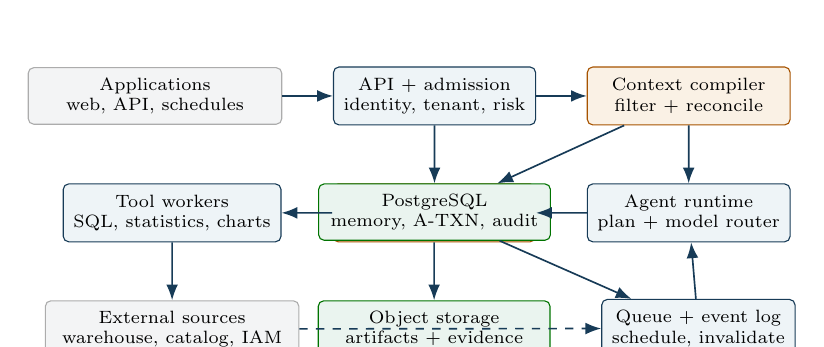
\begin{tikzpicture}[
  scale=0.92,transform shape,
  every node/.style={font=\scriptsize,align=center},
  flow/.style={-Latex,semithick,draw=amosblue},
  box/.style={draw=amosblue,rounded corners=2pt,fill=amoslight,minimum height=8mm,inner sep=4pt},
  gate/.style={draw=orange!65!black,rounded corners=2pt,fill=amosorange,minimum width=28mm,minimum height=8mm,inner sep=3pt},
  store/.style={draw=green!45!black,rounded corners=2pt,fill=amosgreen,minimum width=32mm,inner sep=4pt},
  ext/.style={draw=gray!65,rounded corners=2pt,fill=amosgray,minimum width=35mm,inner sep=4pt}
]
\node[ext] (apps) {Applications\\web, API, schedules};
\node[box,right=7mm of apps] (api) {API + admission\\identity, tenant, risk};
\node[gate,right=7mm of api] (context) {Context compiler\\filter + reconcile};
\node[box,below=8mm of context] (runtime) {Agent runtime\\plan + model router};
\node[gate,left=7mm of runtime] (verify) {Verifier\\pre + post checks};
\node[box,left=7mm of verify] (workers) {Tool workers\\SQL, statistics, charts};
\node[store,below=8mm of api] (state) {PostgreSQL\\memory, A-TXN, audit};
\node[store,below=8mm of verify] (objects) {Object storage\\artifacts + evidence};
\node[ext,below=8mm of workers] (sources) {External sources\\warehouse, catalog, IAM};
\node[box,right=7mm of objects] (events) {Queue + event log\\schedule, invalidate};

\draw[flow] (apps) -- (api);
\draw[flow] (api) -- (context);
\draw[flow] (context) -- (runtime);
\draw[flow] (runtime) -- (verify);
\draw[flow] (verify) -- (workers);
\draw[flow] (workers) -- (sources);
\draw[flow] (api) -- (state);
\draw[flow] (context) -- (state);
\draw[flow] (verify) -- (objects);
\draw[flow] (state) -- (events);
\draw[flow] (events) -- (runtime);
\draw[flow,dashed] (sources) -- (events);
\end{tikzpicture}
\caption{Production logical architecture. Internal boundaries remain explicit even when deployed as one application.}
\label{fig:architecture}
\end{figure}

\subsection{Component Responsibilities}

\begin{table}[ht]
\centering
\scriptsize
\begin{tabularx}{\linewidth}{L{0.18\linewidth}Y Y}
\toprule
\textbf{Component} & \textbf{Owns} & \textbf{Must not own} \\
\midrule
API and admission & Authentication, tenant binding, request validation, idempotency, risk class, quotas. & Prompt construction, warehouse credentials, or final publication logic. \\
Connector manager & Source discovery, version observation, freshness, access probes, change events, read handles. & Cross-source reconciliation or company-wide policy decisions. \\
Memory service & Typed objects, versions, authority, effective time, aliases, supersession, indexes. & Arbitrary raw customer data or model prompts as the system of record. \\
Context compiler & Required-role derivation, policy-first filtering, ranking, reconciliation, compaction, manifest. & Tool execution or hidden fallback when a required role is missing. \\
Agent runtime & Typed planning, model routing, budgets, checkpoints, repair loop, artifact draft. & Credentials, unrestricted tools, or authority to bypass verifier outcomes. \\
Tool workers & Read-only SQL, deterministic statistics, structured charts, result capture; later sandboxed Python behind the same interface. & Long-lived tenant secrets, arbitrary alpha code, or direct publication. \\
Verifier & SQL safety, schema, metrics, freshness, permissions, claim support, risk and review rules. & General truth or causal certainty beyond declared rules. \\
Evidence service & Claims, dependency edges, hashes, verification, artifacts, replay descriptors. & Silent mutation of committed evidence. \\
Scheduler and invalidator & Durable jobs, retries, source-change fan-out, revalidation and review tasks. & Unbounded automatic reruns or publication without current policy. \\
Review application & Evidence inspection, approve/reject/correct, scoped feedback, audit export. & Direct mutation of historical objects or unscoped high-authority feedback. \\
\bottomrule
\end{tabularx}
\caption{Ownership boundaries prevent the language model or any single service from becoming an implicit superuser.}
\end{table}

\section{Product Surfaces and Operating Workflows}

The control plane is useful only when its state is legible to customers. AMOS therefore ships four product surfaces over the same APIs and permission checks; none receives privileged database access.

\begin{table}[ht]
\centering
\small
\begin{tabularx}{\linewidth}{L{0.18\linewidth}L{0.25\linewidth}Y}
\toprule
\textbf{Surface} & \textbf{Primary user} & \textbf{Required capabilities} \\
\midrule
Memory Studio & Data owner and administrator & Connect and test sources; inspect discovered objects and versions; define aliases, metrics, authority, retention, and policies; approve changes; view source health and impact before activation. \\
Analysis Workspace & Analyst and business operator & Submit or schedule a typed task; see admitted scope, plan, budget, progress, warnings, and terminal state; inspect an artifact down to claim, computation, and source; export approved results. \\
Review Queue & Reviewer and domain owner & Compare evidence with the draft; approve, reject, or correct at claim, metric, template, or policy scope; assign effective time and authority; see which future tasks and existing claims are affected. \\
Operations Console & Support, security, and platform operator & Search transactions and audit events; inspect connector, queue, worker, and policy health; retry an idempotent step, revoke a capability, quarantine a connector, revalidate claims, and run recovery procedures. \\
\bottomrule
\end{tabularx}
\caption{The product exposes governed state and explicit controls instead of presenting an opaque chat transcript.}
\end{table}

\subsection{Customer Journey}

Onboarding is an auditable promotion workflow. An administrator creates the tenant, connects a read-only source, confirms identity synchronization, and chooses retention and region. The connector discovers schemas and capabilities into a staging namespace. A data owner resolves aliases, defines or imports a metric, assigns authority, and approves a version. A product owner then configures an application template with task schema, required roles, risk class, review rule, schedule, budget, and artifact shape. Production activation is prohibited until connector, permission, metric, task-fixture, and recovery checks pass.

During normal use, a request or schedule creates a transaction and immediately displays its policy scope. The workspace streams durable state changes rather than model tokens as the source of truth. A user can open the exact context manifest, each execution, each verifier result, and the dependency chain of every material claim. Final status distinguishes \emph{published}, \emph{published with warning}, \emph{awaiting review}, \emph{rejected}, \emph{stale}, and \emph{revoked}; a draft is never visually equivalent to a governed artifact.

After review, corrections append new governed objects and show their scope before confirmation. The next applicable transaction selects them by authority and effective time. Source or policy change computes impact, marks dependent claims, and either revalidates, schedules bounded re-analysis, or requests review. The user can always answer: what changed, what AMOS did, what remains valid, and who has authority to resolve the rest.

\subsection{Experience Invariants}

Every UI action uses the same idempotent API and produces an audit event. Hidden background work has a visible job and owner. Destructive actions are modeled as revocation, supersession, or policy-governed erasure. Restricted object names and failure details are redacted at the API, not merely in the interface. No screen offers a bypass around review, verification, retention, or tenant boundaries.

\section{Data Architecture and Persistent Contracts}

\subsection{Core Relational Model}

Use PostgreSQL as the authoritative store. Object storage holds large artifacts, source exports, chart images, and retained execution payloads. A queue transports durable jobs; it does not replace the transaction log.

\begin{longtable}{L{0.21\linewidth}L{0.26\linewidth}L{0.45\linewidth}}
\toprule
\textbf{Table} & \textbf{Primary identity} & \textbf{Required content and rule} \\
\midrule
\endhead
tenants & tenant\_id & Status, retention policy, encryption key reference, feature gates. Every governed row includes tenant\_id. \\
identities & tenant\_id + subject\_id & Provider, roles, groups, policy attributes, last synchronized epoch. \\
source\_systems & source\_id & Connector type, configuration reference, attainable consistency classes, health. No plaintext secret. \\
memory\_objects & object\_id & Type, logical key, source, authority, permissions, effective interval, recorded time, status, content hash, external reference. \\
memory\_versions & logical\_key + version & Immutable content or reference, source version, transaction time, supersedes link. Updates append; they do not overwrite. \\
alias\_edges & edge\_id & Source-qualified logical identity mapping, authority, effective interval, reviewer state. \\
policies & policy\_id + epoch & Declarative admission, retrieval, tool, publication, retention, and review rules. \\
policy\_decisions & decision\_id & Subject, action, resource, attributes, allow/deny, obligations, policy references, epoch, safe explanation. \\
task\_definitions & task\_type + version & Required/optional roles, consistency minima, tools, claim types, verifier and publication rules, budgets, artifact schema. \\
atxn\_transactions & atxn\_id & Request, identity, risk, budgets, state/state sequence, policy epoch, version vector, timestamps, terminal outcome. \\
context\_manifests & manifest\_id & Selected object versions, required-role coverage, omissions, conflicts, token counts, ranking trace. \\
plans & plan\_id & Typed steps, declared inputs/outputs, tools, budgets, dependencies, model/configuration identity. \\
executions & execution\_id & Capability, worker, tool version, parameters hash, input versions, output reference/hash, latency, cost, status. \\
artifacts & artifact\_id & Type, immutable object reference, audience, risk, creator transaction, object-finalization state. \\
artifact\_publications & publication\_id & Adapter, idempotency key, lifecycle state, external ID, acknowledgment, attempts, revocation state. \\
claims & claim\_id & Typed payload, rendered span, risk, support plan, review state, semantic validity, policy visibility, replay and supersession state. \\
dependency\_edges & edge\_id & Claim-to-query, data, metric, schema, document, execution, feedback, or decision relation. \\
verification\_records & verification\_id & Check type/version, inputs, result, warnings/errors, repairability, timestamp. \\
replay\_packages & package\_id & Replay level, retained inputs, tool/model versions, parameters, hashes, environment descriptor. \\
reviews & review\_id & Reviewer identity, decision, comment, correction scope, authority, affected claims, timestamp. \\
audit\_events & event\_id & Append-only actor, action, target, request/\atxn IDs, outcome, policy epoch, timestamp. \\
jobs & job\_id & Schedule/trigger, idempotency key, state, retry policy, lease, fencing token, next run, dead-letter reason. \\
\bottomrule
\caption{Minimum production schema. JSON payloads may supplement but never replace indexed identity, time, policy, and state columns.}
\end{longtable}

\subsection{Memory Object Contract}

Every memory object must contain a stable ID, source-qualified logical key, type, human-readable summary, structured payload or external reference, source, authority, effective start/end, recorded timestamp, permission labels, sensitivity, version, status, supersedes/superseded-by links, provenance reference, and content hash. Optional confidence cannot override authority.

Write rules are strict. Connectors may write source-observed objects within their namespace. Reviewed corrections may create reviewer-approved feedback. Only designated owners can create owner-approved definitions. Model-inferred memory starts as a hypothesis and cannot govern a high-risk task until approved. Deletion becomes revocation or tombstoning unless a retention policy requires physical erasure.

\subsection{Indexes and Access Paths}

\must The first release uses relational indexes and PostgreSQL full-text search with mandatory tenant and coarse permission predicates. Required indexes include tenant/type/status, logical key/version, effective interval, permission label, source version, authority, supersession, transaction state, job lease, and reverse dependency target. Object-level authorization runs after candidate retrieval. Restricted candidates cannot affect user-visible counts or ranking explanations. Indexes, embedding caches, lexical caches, and object-store keys are tenant-scoped and policy-epoch-aware. \deferred Shared cross-tenant vector indexes. A vector or hybrid backend may later generate candidates only behind the same permission-first interface.

\subsection{Retention and Encryption}

Encrypt transport and storage. Use per-environment keys initially and tenant-specific keys for enterprise isolation. Store secret references in a secret manager. Define retention independently for prompts, model responses, query results, raw evidence, artifacts, audit events, and C2 snapshots. A replay claim is allowed only when the required data remains retained for its declared interval.

\section{Connector Architecture}

Each connector implements a small, testable contract:
\begin{itemize}
  \item \code{discover(scope)} returns source-qualified entities and capabilities;
  \item \code{observe(ref)} returns version, effective time, freshness, sensitivity, access, and consistency class;
  \item \code{read(ref, version, capability)} returns governed content or a bounded read handle;
  \item \code{validate(ref, observed\_version)} confirms whether a C1 observation still holds;
  \item \code{subscribe(cursor)} emits version, schema, permission, freshness, or deletion events;
  \item \code{health()} reports authentication, rate limits, lag, and degraded capabilities.
\end{itemize}

Connector output is untrusted until normalized and policy-labeled. Source text never carries executable policy. Each connector receives least-privilege, tenant-scoped credentials and runs behind egress restrictions. Pagination, retries, backoff, rate-limit state, and source cursors are durable.

\subsection{Connector Build Order}

Build one warehouse adapter first, then identity/policy, semantic definitions, catalog/schema, documents, and event/stream state. Each new adapter must ship with fixtures, contract tests, access-revocation tests, version-change tests, pagination tests, cache-staleness tests, deletion tests, source-outage behavior, and a failure-mode table. C1 certification additionally proves stable version identity, delayed revalidation, overwrite detection, and permission-change observation. C2 additionally proves exact version reads, retention/lease deadlines, expiry behavior, and reconstruction checksums. Do not add a connector solely for breadth; add it when a paid workflow requires one of its roles.

\section{Context Compiler}

The context compiler turns an approved, versioned task definition into a permission-safe working set and an auditable manifest. \must Required roles are stored in \code{task\_definitions}; they are never inferred only by a prompt. The record also freezes consistency minima, allowed tools, claim types, verifier rules, publication requirements, budgets, and artifact schema. Specification C provides the contract.

\subsection{Compilation Algorithm}

\begin{enumerate}
  \item derive required and optional roles from the task type and risk policy;
  \item query candidate indexes with tenant and permission pushdown;
  \item remove inaccessible, revoked, expired, and superseded objects before semantic ranking;
  \item group by source-qualified logical key and resolve aliases explicitly;
  \item reconcile effective time and authority; surface equal-authority conflicts;
  \item choose at least one valid object for every mandatory role;
  \item fill remaining budget by relevance, authority, freshness, verification state, and diversity;
  \item compact only by producing a non-governing derived object with links to every source object;
  \item emit a context manifest containing selections, omissions, conflicts, warnings, token cost, and source versions.
\end{enumerate}

\subsection{Failure Behavior}

Missing role coverage yields \code{needs\_review} or \code{reject}. Ambiguous approved metrics yield a clarification request. Conflicting owner definitions block. Insufficient token budget never silently removes policy, schema, metric, or data-state roles; it drops optional evidence first. Restricted-object counts and identifiers are not revealed to unauthorized users.

\subsection{Compaction Contract}

\must A compacted summary is non-governing evidence, carries the strictest permission scope of every source, links every source version, and is invalidated when any source changes or is revoked. It may not replace a required metric, schema, policy, or data-state object. At most one summary generation may depend on another summary in the first release. Promotion requires measured token reduction and a regression test for factual and permission leakage. \deferred Authority-bearing learned summaries.

\section{Agent Runtime and Tool Execution}

\subsection{Typed Planning}

A plan is data, not free-form prose. Each step declares purpose, required object IDs, tool, parameters schema, expected output, dependency steps, timeout, row/data limits, cost budget, retry policy, verification rules, and review obligation. The runtime validates the plan before any capability is issued.

Model routing is policy-driven. A small classifier may assign task type, a coding model may propose SQL, and a reasoning model may plan an investigation. The stored plan records the exact model provider, model ID, configuration, prompt template version, input manifest, latency, token use, and response hash. Models are replaceable processors; persistent memory and safety controls are not provider-specific.

\subsection{Capabilities and Workers}

The runtime exchanges a plan step for a short-lived, single-purpose capability. A signed capability binds issuer, audience, tenant, \atxn ID, plan step, identity, tool, allowed source and operations, resource limits, issued/not-before/expiry times, unique token ID, policy epoch, and fencing token. Workers reject expired, mismatched, superseded, or replayed capabilities and record the token ID without storing the bearer token.

\must Alpha workers are limited to read-only SQL, deterministic built-in statistics, predefined transformations, and structured chart specifications. SQL workers use source credentials unavailable to the model and enforce approved schemas, statement timeouts, row/byte limits, and query tagging. Every execution writes a hash-addressed result and audit record. \deferred General Python requires a separate sandbox safety case covering image provenance, packages, filesystem, network, secrets, resources, determinism, and replay.

\subsection{Repair Loop}

Repairs are bounded. The verifier may return a machine-readable reason and permitted repair class, such as rename a superseded column or add a required metric predicate. The runtime may attempt at most the policy limit, preserving every failed plan and execution. Permission, policy, or authority failures are never model-repairable.

\section{Verification, Claims, and Publication}

\subsection{Pre-Execution Verification}

For SQL, the verifier parses an AST and checks read-only safety, approved relations and columns, metric-required filters, time semantics, groupings, joins, unsafe functions, row limits, and permission scope. It checks schema version, data freshness, snapshot/watermark state, and whether all referenced objects are in the context manifest. Unsupported constructs produce review or rejection; string matching alone is insufficient.

\subsection{Post-Execution Verification}

After execution, verify result shape, empty or partial outputs, freshness, numeric consistency, denominator rules, uncertainty requirements, chart-data equality, and output sensitivity. \must The alpha constructs typed claims from verified result objects before rendering prose. Each governed template field declares its claim type and support schema; numeric values never originate from model-written text. \deferred Claim extraction from arbitrary prose, notebooks, dashboards, and application payloads is a compatibility feature and cannot be the source of truth.

Claim types include numeric, comparison, trend, forecast, causal, and operational recommendation. Each type has a support plan. Numeric claims require query/result, data state, metric, schema, execution hash, and verification. Causal claims require evidence and remain review-gated unless a pre-approved causal design applies. Recommendations require supporting facts, policy, decision authority, and an explicit reviewer or automation rule.

\subsection{Claim Dependency Graph}

For claim $c$, \amos records edges to computations, data versions, metrics, schemas, documents, feedback, model outputs, verification records, and review decisions:
\begin{equation}
  traceable(c) \not\Rightarrow correct(c) \not\Rightarrow causally\_justified(c).
\end{equation}
The graph proves traceability and supports change impact. Verification supports limited consistency. Causal justification remains a separate methodological judgment.

\subsection{Publication Linearization Point}

Immediately before commit, the runtime revalidates policy epoch and all C1 observations. If any governing state changed, it aborts, repairs, or requests review. The evidence linearization point is the atomic database commit that stores artifact metadata, typed claims, dependencies, verification, replay descriptor, audit event, and object-finalization outbox entry. Large blobs upload first under a temporary key and promote idempotently by content hash.

External dissemination is a separate transaction with explicit forward and revocation paths:
\begin{center}
\scriptsize
\texttt{draft -> prepared -> evidence\_committed -> publication\_pending -> published}\\
\texttt{publication\_pending -> publication\_failed; revocation\_pending -> revoked}
\end{center}
An outbox worker invokes a publication adapter with a stable \idcode{publication_id}; it stores the external identifier and acknowledgment. Lost acknowledgment is recovered by querying or retrying with the same idempotency key, never by creating a second publication. Email, chat, dashboard, ticket, and webhook adapters cannot claim exactly-once behavior unless their target exposes compatible idempotency.

\section{Feedback, Learning, and Invalidation}

Human feedback is a governed state transition. A correction records author, role, authority, scope, effective interval, target artifact/claims, supporting decision, applicability conditions, and provenance. It never silently edits the old artifact. The next applicable context compilation can select the correction according to time, scope, and authority.

Source events trigger reverse dependency traversal. A changed metric, schema, document, permission, or data state identifies affected claims. \must Validity is multidimensional: \code{publication\_validity}, \code{semantic\_validity}, \code{policy\_visibility}, \code{replay\_availability}, \code{review\_state}, and \code{supersession\_state} change independently. Thus a claim can remain historically valid at publication time while becoming semantically stale, hidden from a newly unauthorized viewer, or unreplayable after retention expiry. Fan-out is bounded by tenant quotas, risk priority, deduplication keys, and cooldown windows. External notifications occur only after a new evidence commit and current policy decision.

\subsection{Replay Levels}

\begin{table}[ht]
\centering
\small
\begin{tabularx}{\linewidth}{C{0.08\linewidth}L{0.25\linewidth}Y}
\toprule
\textbf{Level} & \textbf{Promise} & \textbf{Required retention} \\
\midrule
0 & Disposable exploration & Audit event only; no regeneration claim. \\
1 & Evidence reconstruction & Object versions, queries, documents, results, and review records. \\
2 & Artifact regeneration & Level 1 plus structured artifact inputs, templates, and deterministic render configuration. \\
3 & Computational replay & Level 2 plus C2 data, code, parameters, tool environment, and result hashes. \\
4 & Audit package & Level 3 plus policy, identity, approvals, signed manifests, and exportable chain of custody. \\
\bottomrule
\end{tabularx}
\caption{Replay language is precise; model trajectory replay is recorded when possible but is not guaranteed.}
\end{table}

\section{API and Event Contracts}

The first public API is versioned under \code{/v1}. All mutating requests require an idempotency key. Every response includes request ID, \atxn ID where applicable, status, warnings, and a stable error code.

\begin{table}[ht]
\centering
\scriptsize
\begin{tabularx}{\linewidth}{L{0.24\linewidth}L{0.19\linewidth}Y}
\toprule
\textbf{Endpoint} & \textbf{Purpose} & \textbf{Contract} \\
\midrule
POST /tasks & Admit and run or queue analysis & Request/trigger, audience, risk, budgets, required freshness; returns transaction and job IDs. \\
GET /tasks/\{id\} & Observe lifecycle & State, current step, warnings, budgets consumed, review obligation; no hidden restricted details. \\
POST /memory/search & Inspect governed memory & Permission-first typed results and manifest; privileged admin modes are separate. \\
POST /memory & Create governed memory & Authority and source constrained by caller role; append-only version semantics. \\
POST /verify/sql & Preflight proposed SQL & Structured pass/warning/reject, rule IDs, repairability, referenced versions. \\
GET /artifacts/\{id\} & Retrieve artifact metadata & Publication/validity state, audience, evidence links, replay level. \\
POST /artifacts/\{id\}/publications & Request dissemination & Adapter, destination reference, idempotency key; returns publication ID and durable state. \\
GET /publications/\{id\} & Inspect dissemination & Lifecycle, external ID, acknowledgment, attempts, last error, revocation state. \\
GET /claims/\{id\} & Inspect a claim & Exact span, type, support edges, verification, review, current validity. \\
POST /reviews & Approve, reject, or correct & Reviewer identity, scoped decision, affected claims, feedback object created. \\
POST /replay/\{id\} & Reconstruct or replay & Allowed level, retained inputs, status, differences, new audit record. \\
POST /artifacts/\{id\}/revalidate & Check current validity & Traverses dependencies and returns per-claim changes. \\
\bottomrule
\end{tabularx}
\caption{Minimum API surface. Administrative configuration and connector secrets use separate privileged interfaces.}
\end{table}

Events use an envelope containing event ID, type, schema version, tenant, source, subject, occurred/observed times, correlation and \atxn IDs, payload hash, and trace context. Consumers are idempotent. Required event families are:
\begin{itemize}
  \item source and policy: \code{source.version.changed}, \code{policy.epoch.changed}, \code{permission.revoked};
  \item task and evidence: \code{task.state.changed}, \code{artifact.evidence\_committed}, \code{claim.validity\_changed};
  \item dissemination: \idcode{artifact.publication_requested}, \idcode{artifact.published}, \idcode{artifact.publication_failed};
  \item workflow: \code{review.completed}, \code{job.dead\_lettered}.
\end{itemize}

\section{Security and Multi-Tenancy}

\subsection{Trust Boundaries}

Retrieved content, model output, user-provided text, and external tool output are untrusted. Identity tokens, policy decisions, capabilities, source credentials, verification rules, commit logic, and audit events remain outside model text. A successful prompt injection may influence a proposed plan; it must not grant a capability, reveal filtered data, write high-authority memory, or publish restricted output.

\begin{table}[ht]
\centering
\scriptsize
\begin{tabularx}{\linewidth}{L{0.22\linewidth}Y Y}
\toprule
\textbf{Threat} & \textbf{Preventive control} & \textbf{Detection/recovery} \\
\midrule
Cross-tenant leakage & Tenant key on every row, database row-level security, tenant-scoped indexes/keys/caches. & Canary records, access-log analytics, immediate key and token revocation. \\
Indirect prompt injection & Evidence/policy separation, capability checks, sandboxed tools, output validation. & Malicious-content flags, plan diffs, red-team corpus, quarantine. \\
Permission-revocation race & Policy epoch and permission revalidation at commit. & Abort commit, invalidate affected claims, audit event. \\
Memory poisoning & Authority tiers, source namespaces, review gates, immutable versions. & Conflict alerts, provenance inspection, rollback by supersession. \\
Credential exposure & Secret manager, worker-side credential exchange, no secrets in prompts/logs. & Automated scanning, short TTL, rotation and incident runbook. \\
Unsafe SQL or code & AST checks, read-only roles, isolated workers, network/resource limits. & Kill switch, query tags, execution audit, dead-letter evidence. \\
Provenance leakage & Permissioned graph traversal and redacted support views. & Link-access tests, export review, access anomaly alerts. \\
Denial of service & Admission quotas, budgets, concurrency limits, fan-out controls, circuit breakers. & Queue depth/latency alerts, tenant isolation, graceful degradation. \\
\bottomrule
\end{tabularx}
\caption{Security is enforced by external controls, not by asking the model to follow policy.}
\end{table}

\subsection{Policy Decision Contract}

\must Policy is declarative and versioned behind one engine-neutral interface:
\[
evaluate(subject, action, resource, task, environment, epoch)
\rightarrow decision + obligations + policy\_refs.
\]
The persisted result includes allow/deny, row and column constraints, redactions, review and retention obligations, applied policy versions, input-attribute hash, and a caller-safe explanation. Policies may depend on classified result metadata but not arbitrary model prose. Owners author policy drafts; a separate authorized reviewer activates them after simulation against stored decision fixtures. One epoch identifies an immutable set of policy versions. Runtime caches key on tenant, subject attributes, action, resource version, and epoch; epoch activation evicts the prior namespace. The interface permits Rego, Cedar, or a typed internal evaluator, but product code cannot embed bypass policy in prompts or route handlers.

\subsection{Tenant Isolation}

\must Tenant identity appears in every primary key and every foreign-key path through composite keys; no object ID is globally addressable without tenant binding. PostgreSQL row-level security is forced for runtime tables, and runtime roles cannot use \code{BYPASSRLS} or own those tables. Migration and runtime roles are separate. Application repositories repeat tenant predicates; property tests cover cross-tenant joins. Cache keys, indexes, object prefixes, encryption context, queues, capabilities, jobs, and audit queries are tenant-scoped. Canary rows and automated database-policy checks continuously detect bypass. Offer dedicated databases, worker pools, and customer-managed keys when required. Every background job restores tenant context explicitly; missing tenant context is a hard failure.

\subsection{Privacy and Governance}

Minimize retained raw rows. Support field classification, masking, purpose limitation, regional storage, retention, legal hold, export, and erasure. Erasure must update both primary records and derived artifacts while retaining only the minimum audit proof permitted by policy. High-risk model providers receive only the bounded, redacted context allowed by tenant configuration.

\section{Deployment and Scalability Architecture}

\subsection{Initial Production Topology}

Deploy the modular monolith as stateless API/runtime replicas behind a load balancer. Use managed PostgreSQL with point-in-time recovery, object storage with versioning, a managed queue, isolated worker pools, secret manager, identity provider, metrics/logs/traces backend, and a private network path to customer sources. Separate development, staging, and production accounts. Infrastructure is declarative and reviewed.

Run interactive and scheduled workloads in separate queues. Partition workers by tool type and risk. Use \atxn IDs and idempotency keys across retries. Database transactions own state transitions; queue acknowledgements occur only after durable state is written. Long operations renew leases and checkpoints.

\subsection{When to Extract Services}

Do not distribute the system prematurely. Extract a component only when one of these conditions is measured: tool workers require a stronger isolation boundary; connector traffic has independent scaling; context indexes exceed primary-database capacity; invalidation fan-out interferes with interactive latency; enterprise deployment requires separate data planes; or team ownership demands an independent release cycle. Preserve the same typed contracts when extracting.

\subsection{Scaling Strategy}

Scale persistent memory and model context independently. Keep structured filters in the database, move large blobs to object storage, and introduce a dedicated lexical/vector candidate index behind the memory interface when needed. Shard by tenant before sharding within a tenant. Maintain reverse dependency indexes for invalidation. Cache only version-addressed, permission-scoped results; policy-epoch changes evict them.

Capacity planning tracks active tenants, memory objects, version rate, dependency edges, scheduled tasks, tool concurrency, result bytes, model tokens, p50/p95/p99 control-path latency, queue age, and invalidation fan-out. Load tests include one-million-object tenants, policy churn, source delay, and noisy neighbors.

\section{Operations, Reliability, and Support}

\subsection{Service Objectives}

Initial paid-pilot objectives are 99.5\% API availability, 99\% successful scheduled runs excluding declared source outages, p95 admission/context compilation below two seconds at the supported scale, zero confirmed cross-tenant or permission leaks, and 100\% of final artifacts with complete claim/evidence manifests. Objectives tighten only after error budgets and workload shape are understood.

\subsection{Observability}

Every request carries request, \atxn, tenant, job, plan, execution, artifact, publication, and trace IDs. Metrics cover task outcomes, verifier results by rule, context role coverage, retrieval leaks, repair counts, review backlog, capability denials, query cost, model cost, queue age, source health, invalidation lag, publication acknowledgment, replay success, and storage growth. Logs are structured, redacted, immutable according to policy, and linked to traces. Customer-visible status distinguishes \amos failure from source or provider failure.

\subsection{Runbooks}

Ship runbooks for source authentication failure, permission leak suspicion, policy epoch mismatch, stuck transaction, worker compromise, runaway query, queue backlog, database failover, object-store mismatch, invalidation storm, replay mismatch, model-provider outage, and data erasure. Each runbook specifies trigger, containment, customer impact, evidence preservation, recovery, owner, and post-incident tests.

Backups are restored in staging on a schedule. Target RPO is five minutes and RTO is one hour for the control plane during paid pilot, with a longer declared window for reconstructible artifacts. Disaster-recovery drills verify database, object, queue, key, and connector configuration recovery together.

\section{Testing and Quality Gates}

Testing mirrors the architecture rather than only happy-path answers.

\begin{table}[ht]
\centering
\small
\begin{tabularx}{\linewidth}{L{0.20\linewidth}Y Y}
\toprule
\textbf{Layer} & \textbf{Required tests} & \textbf{Release gate} \\
\midrule
Unit/property & Time intervals, authority ordering, supersession, policy evaluation, state transitions, CAS conflicts, fencing, hash stability. & Deterministic and exhaustive boundary cases; mutation/property tests for core invariants. \\
Connector contract & Versions, revocation, pagination, retry, cursor recovery, access denial, rate limit, source deletion. & Same suite passes every connector; no adapter-specific bypass. \\
Context compiler & Role completeness, permission-first filtering, conflicts, ambiguity, budget pressure, compaction lineage. & Zero restricted/superseded selections; mandatory roles never silently dropped. \\
Verifier & Valid/invalid SQL corpus, metrics, schema drift, freshness, unsafe functions, claim support. & Published precision/recall thresholds and zero acceptance of seeded critical violations. \\
End to end & Request, schedule, review, feedback, replay, invalidation, abort/retry, artifact export. & Every terminal outcome and recovery path exercised with persisted evidence. \\
Security & Cross-tenant, prompt injection, poisoning, capability replay, secret leakage, provenance inference, DoS. & Zero critical leaks; red-team findings have regression tests. \\
Reliability & Worker kill, stale lease, database failover, duplicate events, object promotion, lost publication acknowledgment, source timeout, model outage. & No duplicate publication; fenced, idempotent recovery preserves audit trail. \\
Performance & Memory/edge growth, concurrency, churn, fan-out, noisy neighbor, queue saturation. & SLOs hold at declared paid-pilot limits with recorded capacity margin. \\
Human review & Evidence usability, defect detection, correction scope, audit time. & Reviewers can locate support and submit bounded corrections without engineer help. \\
\bottomrule
\end{tabularx}
\caption{A release is not qualified because a demo answer looks correct; each control boundary must pass its own oracle.}
\end{table}

\subsection{Definition of Done for a Feature}

A feature is done only when its typed contract, migration, permissions, audit events, metrics, failure modes, idempotency behavior, retention behavior, tests, operator runbook, and user-facing status are implemented. Model prompt changes alone do not constitute a product feature.

\section{Step-by-Step Build Plan}\label{sec:build-plan}

The team advances by exit gates, not calendar optimism.

\begin{longtable}{L{0.08\linewidth}L{0.15\linewidth}L{0.32\linewidth}L{0.31\linewidth}}
\toprule
\textbf{Phase} & \textbf{Product state} & \textbf{Build} & \textbf{Exit gate} \\
\midrule
\endhead
0 & Architecture foundation & Freeze Specifications A--F, generated schemas, domain types, migrations, \atxn state machine, audit log, tenant/identity skeleton, CI, local fixtures, one-command environment. & Contract examples validate; all invariants have executable tests; a failed step is inspectable and idempotently retryable. \\
1 & Governed memory & Memory/version schema, authority/time/supersession, PostgreSQL search, permission policy, seed tooling, admin inspection. & Permission, time, authority, and supersession property tests pass; no destructive update path. \\
2 & One connector and context & Certified C1 warehouse adapter, versioned task definition, required roles, context compiler, manifest, permission-first search, ambiguity handling. & Frozen task fixtures always include required roles; zero restricted or superseded retrievals; connector certification passes. \\
3 & Governed answer & Typed planner, SQL/statistics/chart workers, capability claims, AST verifier, structured claims, result hashes, report renderer, task API. & At least 90\% safe-and-correct completion on frozen pilot tasks; every numeric claim resolves to evidence. \\
4 & Persistent analyst & Review UI/API, scoped feedback, multidimensional claim validity, replay levels 1--2, schedules, bounded invalidation. & Four weekly shadow cycles complete; corrections affect the next applicable run; validity dimensions change correctly. \\
5 & Paid pilot & SSO/RBAC, defense-in-depth tenancy, object finalization, idempotent publication adapter, durable queues, observability, backups, runbooks, quotas. & Three design partners; zero critical security findings; lost-acknowledgment and recovery drills pass; onboarding under ten business days. \\
6 & Platform API & Stable SDK, connector kit, application templates, model routing, admin controls, retention/erasure, exportable audit packages. & Two independent applications use the same memory/runtime without bespoke core changes. \\
7 & Scale and enterprise & Hybrid indexes, worker/service extraction where measured, dedicated tenancy options, regional deployment, customer-managed keys. & SLOs pass at target tenant/edge/concurrency scale; noisy-neighbor and failover tests pass. \\
8 & Controlled autonomy & Policy-scoped auto-publication, dependency-driven re-analysis, portfolio scheduling, advanced statistics, rollback controls. & Each autonomous task class has a separate safety case, customer approval, monitoring, kill switch, and rollback drill. \\
\bottomrule
\caption{Implementation sequence from empty repository to controlled autonomy.}
\end{longtable}

\subsection{Reference Repository Shape}

Preserve architectural boundaries in code before extracting network services. A practical modular-monolith layout is:

\small
\begin{verbatim}
apps/api/                 admission, public API, event streaming
apps/web/                 Memory Studio, workspace, review, operations
amos/domain/              IDs, value objects, states, errors, interfaces
amos/memory/              objects, versions, authority, time, indexes
amos/connectors/          connector SDK and source adapters
amos/context/             role schemas, selection, reconciliation, manifests
amos/runtime/             planner, controller, budgets, checkpoints, repair
amos/workers/             isolated SQL, statistics, chart workers
amos/verification/        policy, SQL, result, claim, publication checks
amos/evidence/            claims, dependencies, artifacts, replay packages
amos/scheduler/           jobs, leases, retries, invalidation, revalidation
amos/policy/              identity, authorization, risk and retention rules
infra/migrations/         forward database migrations and data backfills
specs/contracts/          generated JSON Schema/OpenAPI and fixtures
specs/conformance/        connector, worker, policy, publication test kits
deploy/                   local, staging, production and recovery definitions
tests/                    unit, contract, integration, security, E2E, load
\end{verbatim}
\normalsize

\begin{samepage}
Dependencies point inward to \texttt{amos/domain}; domain code imports no framework, database driver, model SDK, or connector. Packages call another package through a typed interface and may not write its tables. Transactional state change and an outbox event commit together before asynchronous work begins. External adapters implement ports owned by the calling domain. Architecture tests enforce allowed imports, table ownership, tenant-scoped repositories, and the absence of credentials from model-facing packages.
\end{samepage}

\subsection{First Vertical Slice}

Use a payment-health or subscription-health review as the first commercial workflow. It is recurring, economically meaningful, bounded, and reviewable. Limit the alpha to one metric family, one warehouse, three query shapes, one chart, one report template, and one reviewer role. Shadow the existing analyst process before replacing any deliverable.

The vertical slice is complete when a user request or schedule produces: admitted transaction; versioned context manifest; verified SQL executions; result and chart hashes; structured claims; review-aware report; claim dependencies; replay package; audit trail; and explicit terminal outcome. A fluent report without these records is not an AMOS product slice.

\subsection{Team and Ownership}

A five-person initial team is sufficient: founding architect/product lead; memory/connectors engineer; runtime/tools engineer; product/review engineer; and design-partner/data lead. Assign one named owner for security and operations even if the role is fractional. Every architectural component in Table 3 has a code owner and operational owner before paid pilot.

\section{Current Prototype to Production}

The repository already demonstrates useful seams: Python domain models, SQLite-backed memory, permission filtering, temporal/authority reconciliation, a planner/controller, DuckDB execution, SQL verification, claim provenance, replay, FastAPI routes, scenarios, and an 85-test regression suite. This proves the vertical control loop can run. It is not yet the complete production architecture.

\begin{table}[ht]
\centering
\scriptsize
\begin{tabularx}{\linewidth}{L{0.22\linewidth}Y Y}
\toprule
\textbf{Area} & \textbf{Prototype} & \textbf{Production completion work} \\
\midrule
State store & SQLite tables and local artifacts. & PostgreSQL migrations, row-level security, HA, PITR, object storage, retention, tenant keys. \\
Transactions & Controller sequence and audit records. & Explicit \atxn state machine, CAS transitions, fencing, policy/source revalidation, outbox, atomic evidence commit. \\
Connectors & Synthetic DuckDB and fixture-shaped adapters. & Versioned connector SDK, real warehouse/IAM/semantic/document adapters, change subscriptions. \\
Runtime & One payment workflow and templated plan. & Versioned task definitions, typed plans, model router, durable checkpoints, signed capabilities, SQL/statistics/chart workers, repair budgets. \\
Verification & Read-only SQL, schema, metric, freshness, permissions, provenance. & Supported SQL fragment spec, result/statistical checks, rule versioning, claim-type policies, false-reject monitoring. \\
Provenance & Claim records, support links, replay hashes. & Structured claim schemas, general dependency graph, review decisions, validity dimensions, reverse invalidation, signed audit export. \\
API & FastAPI task/memory/claim/artifact/replay routes. & Versioning, idempotency, publication lifecycle, pagination, quotas, stable error taxonomy, event schemas, SDK. \\
Operations & Local execution and evaluation harness. & Queue, observability, SLOs, on-call, backups, DR, metering, customer status, incident runbooks. \\
Security & Permission filters and read-only tools. & SSO/RBAC, tenant isolation, secret manager, worker sandbox, egress controls, red-team program. \\
\bottomrule
\end{tabularx}
\caption{The production plan extends the existing prototype without confusing local feasibility with a deployable product.}
\end{table}

\section{Architecture Decisions and Non-Goals}

Key decisions are explicit:
\begin{itemize}
  \item build a modular monolith first, with internal service contracts and one authoritative transaction database;
  \item keep raw data in source systems and move bounded results or retained snapshots only under policy;
  \item enforce permissions before retrieval ranking and again at execution and commit;
  \item treat models as untrusted, replaceable processors with no ambient credentials;
  \item use optimistic cross-source validation rather than claim nonexistent global ACID guarantees;
  \item attach provenance at claim granularity and define replay levels precisely;
  \item construct typed claims before prose and persist validity dimensions separately;
  \item separate evidence commit, object finalization, and external dissemination;
  \item gate causal and high-impact conclusions on human or approved methodological review;
  \item add autonomy per task class, never as a platform-wide switch.
\end{itemize}

\deferred General Python, free-form claim extraction, vector retrieval, and automatic external publication. \nongoal Universal enterprise knowledge management, unrestricted natural-language access to all data, arbitrary production writes, perfect model reproducibility, automatic causal discovery, and replacing warehouses, semantic layers, catalogs, lineage systems, or BI tools.

\section{Harsh Qualification Checklist}

Before claiming that AMOS is ready for a paid pilot, answer yes to every item:
\begin{enumerate}
  \item Can an operator reconstruct why every selected memory object entered the context and why every omitted mandatory role caused a visible outcome?
  \item Can permission revocation between retrieval and publication prevent commit without relying on the model?
  \item Can every numeric statement in a final artifact resolve to query, result hash, data version, metric, schema, and verification?
  \item Can a reviewer correction affect the next applicable task while the original artifact remains immutable?
  \item Can a metric or schema change identify and reclassify every dependent claim?
  \item Can duplicate requests, events, or retries occur without duplicate publication?
  \item Can a worker be killed or compromised without exposing long-lived credentials or corrupting transaction history?
  \item Can the team restore database, objects, queue state, keys, and connector configuration within the declared RTO?
  \item Can a tenant export its audit package and enforce retention or erasure without another tenant being observable?
  \item Can a lost publication acknowledgment be retried without creating a duplicate external artifact?
  \item Do composite tenant keys, forced RLS, repositories, caches, object paths, and capabilities all reject cross-tenant access?
  \item Can model provider, retrieval backend, or worker implementation change without changing the memory and \atxn contracts?
  \item Do load, security, connector, failure-injection, and human-review tests pass at the declared supported scale?
  \item Does the product save measurable analyst/reviewer time while maintaining zero confirmed critical permission leaks?
\end{enumerate}

A no answer is an architectural gap, not documentation debt. The corresponding phase remains incomplete until the gap has an owner, contract, test, metric, and runbook.

\section{Conclusion}

\amos becomes a product when persistent company knowledge, model reasoning, tool execution, verification, human judgment, and artifacts are joined by one enforceable operating contract. Typed analytical memory provides durable state. The bounded context compiler supplies only valid and permitted working memory. \atxn makes admission, version observation, capabilities, validation, commit, dissemination, replay, and invalidation explicit. Claim dependencies make conclusions inspectable and change-aware. External enforcement keeps models useful without making them trusted authorities.

The implementation path is deliberately practical: build one governed read-only workflow in a modular monolith; make every outcome and dependency observable; add durable review, scheduling, tenancy, operations, and connector breadth; then introduce platform APIs and autonomy only when phase-specific gates pass. If the team follows the contracts and qualification checklist in this guide, it can build AMOS end to end without leaving the hardest correctness, security, and operational decisions implicit.

\clearpage
\appendix

\section{Specification A: A-TXN, Concurrency, and Publication}

This specification freezes the internal state machine and the boundary between evidence commit, object finalization, and external dissemination. Generated enums and transition tests must match this section.

\subsection{Persistent State Machine}

\begin{longtable}{L{0.17\linewidth}L{0.26\linewidth}L{0.49\linewidth}}
\toprule
\textbf{Current state} & \textbf{Allowed next state} & \textbf{Required guard and durable effect} \\
\midrule
\endhead
admitted & observing, rejected & Identity, tenant, task definition, risk, budgets, policy epoch, and request idempotency key are fixed. \\
observing & selecting, needs\_review, aborted & Required connector observations and attainable consistency classes are stored. \\
selecting & planning, needs\_review, rejected & Manifest covers every required role; omissions and conflicts are explicit. \\
planning & executing, needs\_review, rejected & Typed plan validates against the task definition and budget. \\
executing & composing, repairing, aborted & Every execution uses the current lease fence and a valid capability; results are hash-addressed. \\
repairing & executing, needs\_review, rejected & Failure is in an allowed repair class and the attempt budget remains. \\
composing & verifying, aborted & Typed claims and artifact inputs are stored before prose render. \\
verifying & revalidating, repairing, needs\_review, rejected & Versioned verifier results cover every required rule and claim. \\
revalidating & evidence\_committed, repairing, needs\_review, rejected, aborted & Policy epoch, C1 observations, C2 leases, task version, and publication obligations still hold. \\
evidence\_committed & object\_finalizing, publication\_pending, needs\_review & Claims, dependencies, replay descriptor, audit event, and outbox records commit atomically. \\
object\_finalizing & publication\_pending, object\_failed & Temporary objects promote by content hash; mismatch never mutates committed evidence. \\
publication\_pending & published, publication\_failed & Adapter receives stable publication ID and stores external acknowledgment or classified failure. \\
published & revocation\_pending & Only policy, review, or invalidation may request revocation; evidence remains immutable. \\
revocation\_pending & revoked, publication\_failed & Adapter records target acknowledgment; retries retain the same publication ID. \\
needs\_review & verifying, revalidating, rejected & A current authorized review supplies the exact missing obligation. \\
rejected, aborted, revoked & none & Terminal outcome and evidence are immutable; a retry creates or resumes only through an explicit retry record. \\
\bottomrule
\caption{Allowed \atxn and publication transitions. A generated transition matrix is the implementation source of truth.}
\end{longtable}

\subsection{Isolation, Compare-and-Swap, and Fencing}

\must Each database interaction is a short PostgreSQL \code{READ COMMITTED} transaction. Transition code performs compare-and-swap on tenant, \atxn ID, current state, and \code{state\_seq}; success increments the sequence. A zero-row update means a concurrency conflict, not success.

\begin{lstlisting}[style=contract]
UPDATE atxn_transactions
SET state = :next_state,
    state_seq = state_seq + 1,
    updated_at = clock_timestamp()
WHERE tenant_id = :tenant_id
  AND atxn_id = :atxn_id
  AND state = :expected_state
  AND state_seq = :expected_seq
  AND terminal = false;
\end{lstlisting}

Job acquisition uses \code{SELECT ... FOR UPDATE SKIP LOCKED}, increments \code{fencing\_token}, and commits before work begins. Every checkpoint, execution, object promotion, outbox completion, and publication attempt compares that fence. A renewed lease never reuses an old fence. Terminal records reject updates at both repository and database layers. Review, invalidation, and publication commands lock the affected artifact row and compare its validity sequence before appending a new state.

\must Every mutation and its outbox event share one database commit. Event consumers deduplicate by tenant and event ID. Side effects use the stable key \code{tenant/atxn/step/effect}; publication uses \code{tenant/publication\_id}. Duplicate requests return the original resource when the request hash matches and return \code{IDEMPOTENCY\_CONFLICT} when it differs.

\subsection{Normal Task and Commit-Time Revocation}

\begin{figure}[H]
\centering
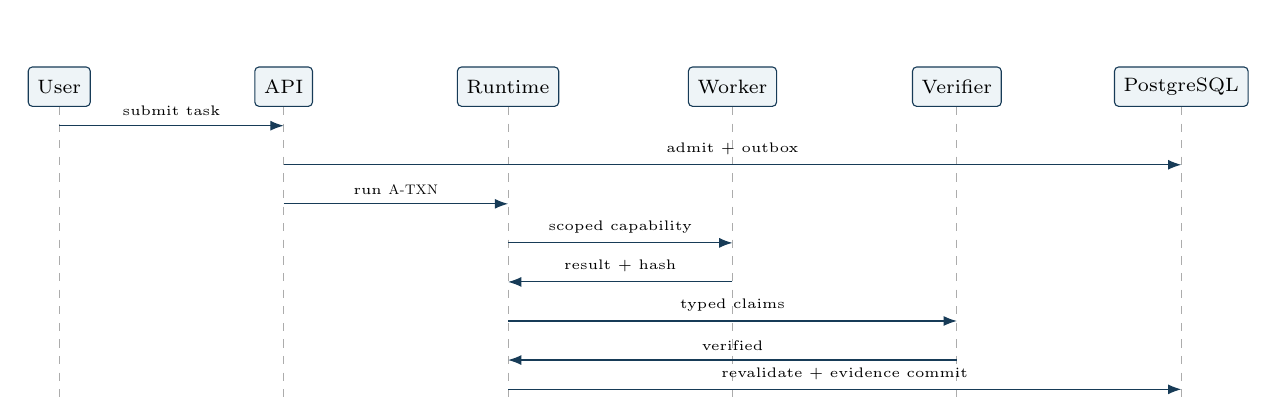
\begin{tikzpicture}[x=0.95cm,y=0.62cm]
\node[seqactor] (u) at (0,0) {User};
\node[seqactor] (a) at (3,0) {API};
\node[seqactor] (r) at (6,0) {Runtime};
\node[seqactor] (w) at (9,0) {Worker};
\node[seqactor] (v) at (12,0) {Verifier};
\node[seqactor] (d) at (15,0) {PostgreSQL};
\foreach \n in {u,a,r,w,v,d}{\draw[seqlife] (\n.south) -- ++(0,-6.3);}
\draw[seqmsg] (0,-0.8)--node[above,font=\tiny]{submit task}(3,-0.8);
\draw[seqmsg] (3,-1.6)--node[above,font=\tiny]{admit + outbox}(15,-1.6);
\draw[seqmsg] (3,-2.4)--node[above,font=\tiny]{run \atxn}(6,-2.4);
\draw[seqmsg] (6,-3.2)--node[above,font=\tiny]{scoped capability}(9,-3.2);
\draw[seqmsg] (9,-4.0)--node[above,font=\tiny]{result + hash}(6,-4.0);
\draw[seqmsg] (6,-4.8)--node[above,font=\tiny]{typed claims}(12,-4.8);
\draw[seqmsg] (12,-5.6)--node[above,font=\tiny]{verified}(6,-5.6);
\draw[seqmsg] (6,-6.2)--node[above,font=\tiny]{revalidate + evidence commit}(15,-6.2);
\end{tikzpicture}
\caption{Normal task lifecycle. Durable state, not streamed model text, advances the product.}
\end{figure}

\begin{figure}[H]
\centering
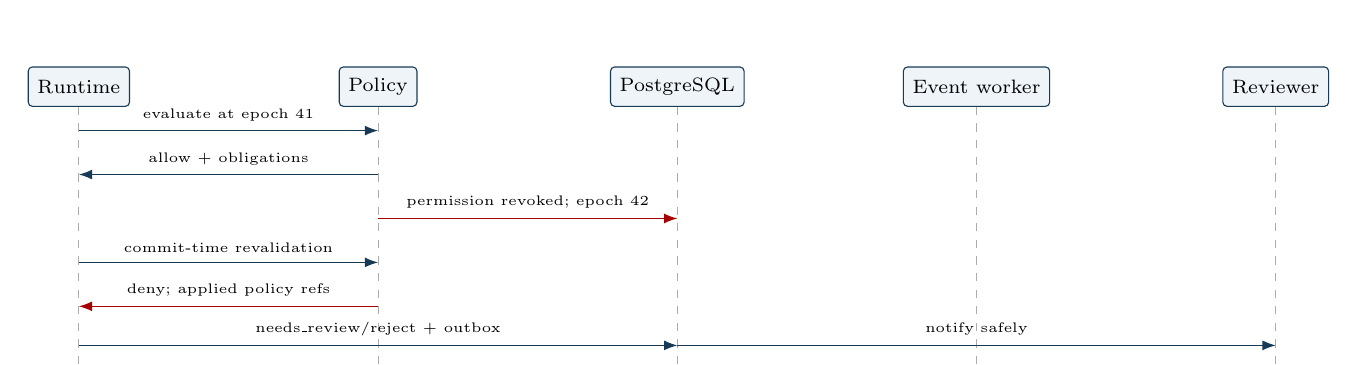
\begin{tikzpicture}[x=0.95cm,y=0.62cm]
\node[seqactor] (r) at (0,0) {Runtime};
\node[seqactor] (p) at (4,0) {Policy};
\node[seqactor] (d) at (8,0) {PostgreSQL};
\node[seqactor] (e) at (12,0) {Event worker};
\node[seqactor] (u) at (16,0) {Reviewer};
\foreach \n in {r,p,d,e,u}{\draw[seqlife] (\n.south) -- ++(0,-5.5);}
\draw[seqmsg] (0,-0.9)--node[above,font=\tiny]{evaluate at epoch 41}(4,-0.9);
\draw[seqmsg] (4,-1.8)--node[above,font=\tiny]{allow + obligations}(0,-1.8);
\draw[seqfail] (4,-2.7)--node[above,font=\tiny]{permission revoked; epoch 42}(8,-2.7);
\draw[seqmsg] (0,-3.6)--node[above,font=\tiny]{commit-time revalidation}(4,-3.6);
\draw[seqfail] (4,-4.5)--node[above,font=\tiny]{deny; applied policy refs}(0,-4.5);
\draw[seqmsg] (0,-5.3)--node[above,font=\tiny]{needs\_review/reject + outbox}(8,-5.3);
\draw[seqmsg] (8,-5.3)--node[above,font=\tiny]{notify safely}(16,-5.3);
\end{tikzpicture}
\caption{Commit-time policy revocation prevents publication without relying on the model.}
\end{figure}

\subsection{External Publication Protocol}

The publication adapter interface is \code{prepare}, \code{publish}, \code{status}, and \code{revoke}. \code{prepare} validates destination, audience, current policy, and payload hash without a side effect. \code{publish} accepts a stable publication ID. \code{status} reconciles lost acknowledgment. \code{revoke} is idempotent and records whether the target can truly retract or only append a correction. Permanent failures move to dead letter with operator ownership; retryable failures use capped exponential backoff and preserve the same ID.

\begin{figure}[H]
\centering
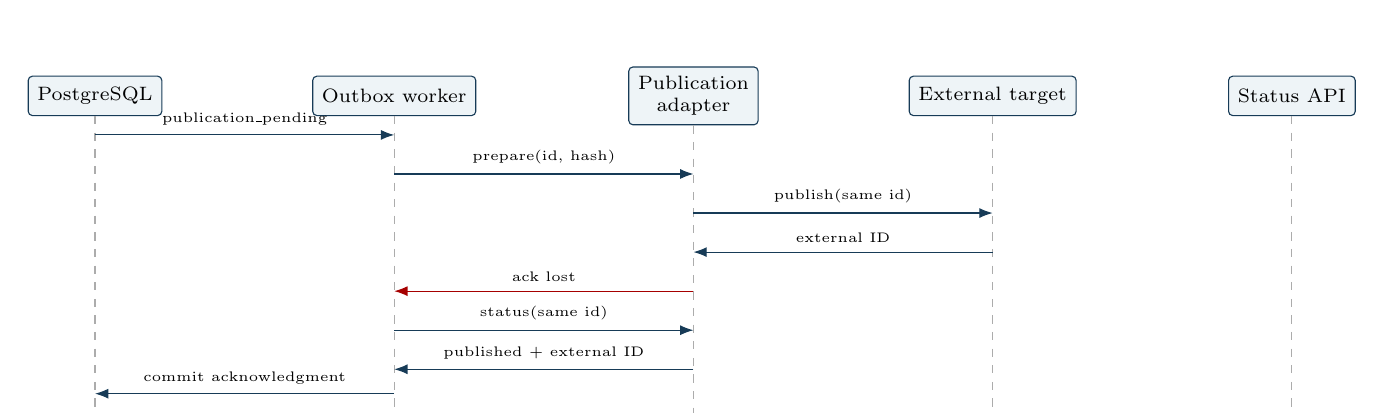
\begin{tikzpicture}[x=0.95cm,y=0.62cm]
\node[seqactor] (d) at (0,0) {PostgreSQL};
\node[seqactor] (o) at (4,0) {Outbox worker};
\node[seqactor] (a) at (8,0) {Publication\\adapter};
\node[seqactor] (t) at (12,0) {External target};
\node[seqactor] (s) at (16,0) {Status API};
\foreach \n in {d,o,a,t,s}{\draw[seqlife] (\n.south) -- ++(0,-6.1);}
\draw[seqmsg] (0,-0.8)--node[above,font=\tiny]{publication\_pending}(4,-0.8);
\draw[seqmsg] (4,-1.6)--node[above,font=\tiny]{prepare(id, hash)}(8,-1.6);
\draw[seqmsg] (8,-2.4)--node[above,font=\tiny]{publish(same id)}(12,-2.4);
\draw[seqmsg] (12,-3.2)--node[above,font=\tiny]{external ID}(8,-3.2);
\draw[seqfail] (8,-4.0)--node[above,font=\tiny]{ack lost}(4,-4.0);
\draw[seqmsg] (4,-4.8)--node[above,font=\tiny]{status(same id)}(8,-4.8);
\draw[seqmsg] (8,-5.6)--node[above,font=\tiny]{published + external ID}(4,-5.6);
\draw[seqmsg] (4,-6.1)--node[above,font=\tiny]{commit acknowledgment}(0,-6.1);
\end{tikzpicture}
\caption{External publication recovers a lost acknowledgment without duplicating the target artifact.}
\end{figure}

\section{Specification B: Persistent Model and Database Invariants}

\subsection{Keys, Constraints, and Roles}

\begin{longtable}{L{0.24\linewidth}L{0.68\linewidth}}
\toprule
\textbf{Invariant} & \textbf{Implementation rule} \\
\midrule
\endhead
Tenant binding & Every primary key and foreign key includes \code{tenant\_id}. Lookups require tenant plus local ID. Composite foreign keys prevent cross-tenant references. \\
Forced RLS & Runtime tables enable and force row-level security. Runtime roles neither own tables nor hold \code{BYPASSRLS}; migration roles are separate and unavailable to the application. \\
Immutability & Memory versions, executions, evidence commits, claims, dependencies, reviews, and audit events are append-only. Correction uses supersession or a new validity record. \\
State checks & Database checks constrain enum values, nonnegative budgets, effective intervals, terminal flags, and publication transition pairs. Repository CAS supplies transition legality. \\
Version identity & Unique constraints cover tenant, source, logical key, source version, and content hash where appropriate. Equal version with unequal content is a connector incident. \\
Idempotency & Unique tenant-scoped keys exist for requests, events, executions, object promotions, jobs, reviews, and publication attempts. \\
Ownership & Each package owns its tables; other packages use typed ports. Direct cross-package writes fail architecture tests and database grants. \\
Audit & Sensitive changes append actor, action, target, decision, policy epoch, request, \atxn, correlation, and time. Audit payloads are redacted but tamper-evident. \\
\bottomrule
\caption{Database invariants are repeated at schema, database-role, repository, and test layers.}
\end{longtable}

Required indexes begin with tenant and cover active logical version, effective interval, authority, permission label, source version, \atxn state sequence, job readiness/lease, publication state, and reverse dependency target. A migration that changes a state or contract ships with forward DDL, bounded backfill, compatibility window, verification query, rollback or roll-forward plan, and observed capacity cost. Destructive column removal waits until all running application versions stop reading it.

\Needspace{0.55\textheight}
\subsection{Example A-TXN Record}

\begin{lstlisting}[style=contract]
{
  "tenant_id": "ten_01",
  "atxn_id": "atxn_01J2",
  "task_definition": {"type": "payment_health_review", "version": 3},
  "request_hash": "sha256:...",
  "subject_id": "usr_42",
  "risk": "material_internal",
  "state": "revalidating",
  "state_seq": 12,
  "policy_epoch": 41,
  "source_versions": {
    "metric:payment_failure_rate": "v3",
    "schema:payments": "etag:82ab",
    "snapshot:warehouse": "snap_2026_07_12T1900Z"
  },
  "manifest_id": "ctx_91",
  "plan_id": "plan_17",
  "fencing_token": 8,
  "outcome": null,
  "created_at": "2026-07-12T19:02:11Z",
  "updated_at": "2026-07-12T19:03:27Z"
}
\end{lstlisting}

\subsection{Object Finalization and Retention}

Temporary objects use a tenant prefix and a random upload ID. The evidence commit stores expected hash, size, media type, retention class, and final content-addressed key. Promotion copies or renames idempotently, verifies hash and encryption context, then appends finalization state. A mismatch quarantines the temporary object and leaves evidence inspectable but non-publishable. Garbage collection deletes unreferenced temporary objects only after the maximum retry window.

Retention evaluates each evidence class independently. Erasure creates a tombstone, removes primary and derived bytes, invalidates dependent summaries, and retains only the minimum policy-permitted proof. C2 leases record expiry and renewal; replay availability changes when a lease expires even if historical publication validity remains true.

\Needspace{0.55\textheight}
\section{Specification C: Task Definitions and Context Manifests}

\subsection{Versioned Task Definition}

\begin{lstlisting}[style=contract]
task_type: payment_health_review
version: 3
status: approved
risk_class: material_internal
required_roles:
  - metric_definition
  - active_schema
  - data_snapshot
  - user_policy
  - review_policy
optional_roles:
  - prior_incident
  - deployment_event
  - reviewer_feedback
minimum_consistency:
  metric_definition: C1
  active_schema: C1
  data_snapshot: C2
  user_policy: C1
allowed_tools:
  - sql.readonly.v1
  - stats.rate_comparison.v1
  - chart.timeseries.v1
claim_types:
  - metric_value
  - metric_comparison
  - operational_recommendation
verifier_profile: payment_health.v2
publication_policy: human_review_required
budgets: {max_steps: 8, max_repairs: 2, max_rows: 50000}
artifact_schema: payment_health_report.v3
\end{lstlisting}

Task definitions are immutable after approval. A new version declares compatibility, migration behavior for schedules, fixture corpus, owner, reviewer, effective interval, and superseded version. Admission binds one version for the entire \atxn. Dynamic policy may add obligations or deny execution but cannot silently remove required roles or verifier rules.

\Needspace{0.55\textheight}
\subsection{Example Context Manifest}

\begin{lstlisting}[style=contract]
{
  "manifest_id": "ctx_91",
  "tenant_id": "ten_01",
  "atxn_id": "atxn_01J2",
  "task_definition": "payment_health_review:v3",
  "policy_epoch": 41,
  "required_role_coverage": {
    "metric_definition": ["mem_metric_pfr_v3"],
    "active_schema": ["mem_schema_payments_82ab"],
    "data_snapshot": ["mem_snapshot_1900"],
    "user_policy": ["mem_policy_access_41"],
    "review_policy": ["mem_policy_review_9"]
  },
  "optional_selected": ["mem_incident_217"],
  "omissions": [{"role": "deployment_event", "reason": "no_authorized_candidate"}],
  "conflicts": [],
  "token_count": 6840,
  "source_versions": ["metric:v3", "schema:82ab", "snapshot:1900"],
  "ranking_trace_ref": "obj://ten_01/traces/ctx_91"
}
\end{lstlisting}

\subsection{Selection and Compaction Rules}

Candidate SQL always applies tenant, active status, effective-time overlap, coarse permission scope, and non-superseded filters before text ranking. Object authorization then evaluates the exact subject and policy epoch. The response reveals neither pre-authorization count nor restricted candidate identity. A cache entry is keyed by tenant, task version, subject-attribute hash, policy epoch, query hash, and source-version vector.

Required roles select valid governing objects before optional relevance ranking. Equal-authority conflicts block. Budget pressure removes optional evidence first. A compacted object inherits the strictest source permission and shortest retention, is non-governing, links all source versions, is invalidated on any source change, and cannot satisfy metric, schema, policy, or data-state roles.

\Needspace{0.55\textheight}
\section{Specification D: Connector SDK and Certification}

\subsection{Typed Connector Interface}

\begin{lstlisting}[style=contract]
discover(scope, cursor?) -> Page<EntityRef>
observe(ref) -> Observation {
  source_version, observed_at, effective_interval,
  freshness, sensitivity, access_descriptor,
  consistency_class, retention_deadline?
}
read(ref, source_version, capability) -> BoundedHandle
validate(ref, source_version) -> Validation {same, current_version, reason}
subscribe(cursor) -> Page<SourceEvent>
health() -> Health {status, lag, rate_limit, degraded_capabilities}
\end{lstlisting}

Version identity must represent content or source transaction state strongly enough for the advertised class. Connector configuration declares whether updates overwrite identities, how deletions and permission changes surface, cache behavior, clock assumptions, pagination consistency, cursor expiry, and source outage semantics. Equal source version with different normalized content is a hard incident.

\subsection{Certification Matrix}

\begin{longtable}{L{0.22\linewidth}C{0.09\linewidth}C{0.09\linewidth}C{0.09\linewidth}L{0.30\linewidth}}
\toprule
\textbf{Behavior} & \textbf{C0} & \textbf{C1} & \textbf{C2} & \textbf{Oracle} \\
\midrule
\endhead
Stable observation identity & required & required & required & Repeated observation without change returns equal version. \\
Delayed revalidation & --- & required & required & Change after delay returns unequal version or unavailable. \\
Overwrite and deletion & observed & required & required & Fixture overwrite/deletion cannot validate old state. \\
Permission change & observed & required & required & Revocation becomes observable within declared bound. \\
Pagination/cursor recovery & required & required & required & No silent duplicate, omission, or cross-scope item. \\
Cache staleness bound & declared & enforced & enforced & Bypass/expiry test meets declared maximum. \\
Exact version read & --- & optional & required & Old version reads exact bytes and checksum. \\
Retention lease & --- & --- & required & Deadline, renewal, expiry, and missing snapshot are deterministic. \\
Source unavailable & required & required & required & Returns classified unavailable, never a guessed validation. \\
\bottomrule
\caption{A connector earns its consistency class through conformance tests, not self-description.}
\end{longtable}

\Needspace{0.55\textheight}
\subsection{Example Source-Change Event}

\begin{lstlisting}[style=contract]
{
  "event_id": "evt_src_882",
  "schema_version": 1,
  "type": "source.version.changed",
  "tenant_id": "ten_01",
  "source_id": "warehouse_primary",
  "subject": "schema:payments",
  "previous_version": "etag:82ab",
  "current_version": "etag:91cc",
  "change_kind": "schema",
  "occurred_at": "2026-07-12T20:00:00Z",
  "observed_at": "2026-07-12T20:00:09Z",
  "cursor": "cur_10921",
  "deduplication_key": "warehouse_primary/schema:payments/etag:91cc"
}
\end{lstlisting}

\section{Specification E: Workers, Capabilities, and Verification}

\subsection{Capability Claims}

\begin{lstlisting}[style=contract]
{
  "iss": "amos-runtime",
  "aud": "sql-worker",
  "tenant_id": "ten_01",
  "atxn_id": "atxn_01J2",
  "plan_id": "plan_17",
  "step_id": "step_03",
  "subject_id": "usr_42",
  "tool": "sql.readonly.v1",
  "source_id": "warehouse_primary",
  "operations": ["query"],
  "relations": ["analytics.payments"],
  "limits": {"seconds": 30, "rows": 50000, "bytes": 5000000},
  "policy_epoch": 41,
  "fencing_token": 8,
  "jti": "cap_7701",
  "nbf": 1783908200,
  "exp": 1783908260
}
\end{lstlisting}

Capabilities are signed by a dedicated issuer, audience-bound, short-lived, single-use for side-effecting operations, and exchanged only over authenticated worker channels. The worker fetches source credentials from the secret broker after capability validation; the model and runtime plan never receive them. Audit stores token ID and claims hash, not the bearer token.

\Needspace{0.55\textheight}
\subsection{Typed Plan and Verifier Result}

\begin{lstlisting}[style=contract]
{
  "plan_id": "plan_17",
  "task_definition": "payment_health_review:v3",
  "manifest_id": "ctx_91",
  "steps": [{
    "step_id": "step_03",
    "purpose": "compute current and baseline failure rates",
    "tool": "sql.readonly.v1",
    "input_object_ids": ["mem_metric_pfr_v3", "mem_schema_payments_82ab"],
    "parameter_schema": "payment_rate_query.v2",
    "expected_output_schema": "rate_comparison.v1",
    "timeout_seconds": 30,
    "limits": {"rows": 50000, "bytes": 5000000},
    "retry": {"max_attempts": 2, "repair_classes": ["COLUMN_SUPERSEDED"]},
    "verifier_profile": "payment_health.v2"
  }]
}
\end{lstlisting}

\begin{lstlisting}[style=contract]
{
  "verification_id": "ver_551",
  "execution_id": "exec_123",
  "verifier_profile": "payment_health.v2",
  "profile_version": 2,
  "outcome": "pass",
  "checks": [
    {"rule_id": "SQL_READ_ONLY", "outcome": "pass"},
    {"rule_id": "METRIC_FILTERS", "outcome": "pass"},
    {"rule_id": "SCHEMA_VERSION", "outcome": "pass"},
    {"rule_id": "RESULT_DENOMINATOR", "outcome": "pass"}
  ],
  "warnings": [],
  "permitted_repair": null,
  "input_hash": "sha256:...",
  "created_at": "2026-07-12T19:03:11Z"
}
\end{lstlisting}

\subsection{Worker Protocol and Deferred Python}

The worker validates capability signature, audience, time, tenant, source, operation, policy epoch, and fence; reserves the execution idempotency key; obtains a short-lived source credential; validates the operation; executes within limits; writes result bytes under a temporary tenant key; commits output hash and classified status; destroys credentials; and acknowledges only after durable state. Cancellation and lease loss stop execution and prohibit commit.

\deferred A general Python worker is not an alpha component. Its later safety case must define immutable runtime images, allowlisted packages and hashes, no ambient network or filesystem, secret absence, syscall and resource isolation, data-egress controls, deterministic seed/time behavior, result capture, vulnerability response, and replay claims.

\subsection{Verifier Repair and Worker Crash Sequences}

\begin{figure}[H]
\centering
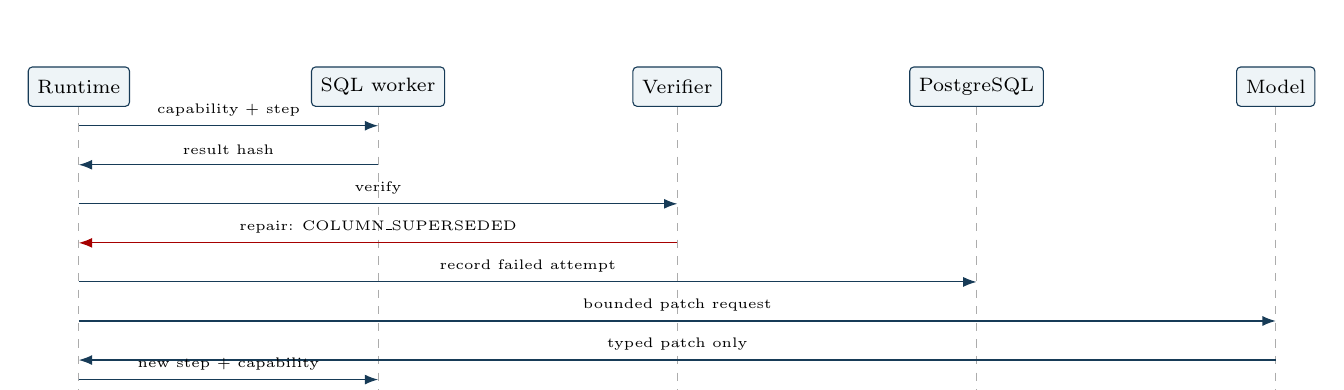
\begin{tikzpicture}[x=0.95cm,y=0.62cm]
\node[seqactor] (r) at (0,0) {Runtime};
\node[seqactor] (w) at (4,0) {SQL worker};
\node[seqactor] (v) at (8,0) {Verifier};
\node[seqactor] (d) at (12,0) {PostgreSQL};
\node[seqactor] (m) at (16,0) {Model};
\foreach \n in {r,w,v,d,m}{\draw[seqlife] (\n.south) -- ++(0,-6);}
\draw[seqmsg] (0,-0.8)--node[above,font=\tiny]{capability + step}(4,-0.8);
\draw[seqmsg] (4,-1.6)--node[above,font=\tiny]{result hash}(0,-1.6);
\draw[seqmsg] (0,-2.4)--node[above,font=\tiny]{verify}(8,-2.4);
\draw[seqfail] (8,-3.2)--node[above,font=\tiny]{repair: COLUMN\_SUPERSEDED}(0,-3.2);
\draw[seqmsg] (0,-4.0)--node[above,font=\tiny]{record failed attempt}(12,-4.0);
\draw[seqmsg] (0,-4.8)--node[above,font=\tiny]{bounded patch request}(16,-4.8);
\draw[seqmsg] (16,-5.6)--node[above,font=\tiny]{typed patch only}(0,-5.6);
\draw[seqmsg] (0,-6.0)--node[above,font=\tiny]{new step + capability}(4,-6.0);
\end{tikzpicture}
\caption{Verifier repair is bounded, typed, and preserves the failed attempt.}
\end{figure}

\begin{figure}[H]
\centering
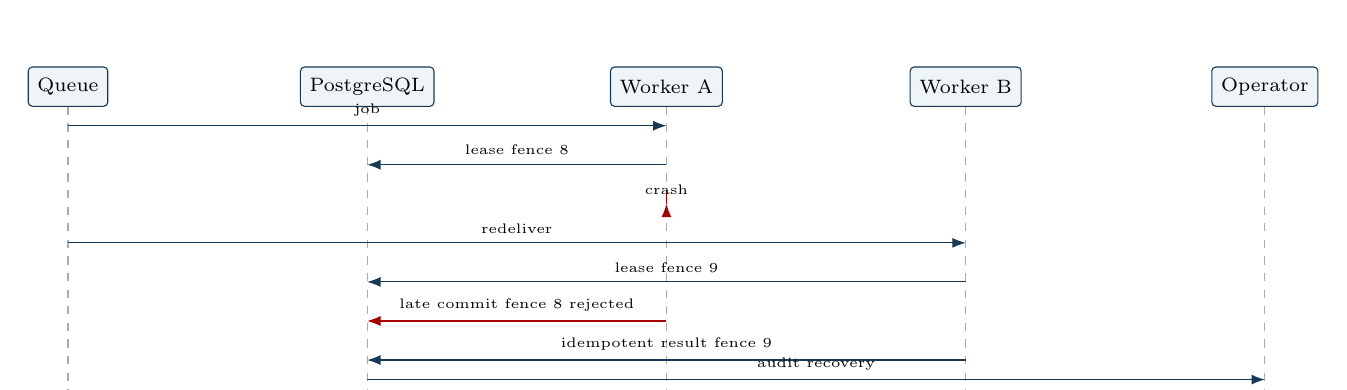
\begin{tikzpicture}[x=0.95cm,y=0.62cm]
\node[seqactor] (q) at (0,0) {Queue};
\node[seqactor] (d) at (4,0) {PostgreSQL};
\node[seqactor] (w1) at (8,0) {Worker A};
\node[seqactor] (w2) at (12,0) {Worker B};
\node[seqactor] (o) at (16,0) {Operator};
\foreach \n in {q,d,w1,w2,o}{\draw[seqlife] (\n.south) -- ++(0,-6);}
\draw[seqmsg] (0,-0.8)--node[above,font=\tiny]{job}(8,-0.8);
\draw[seqmsg] (8,-1.6)--node[above,font=\tiny]{lease fence 8}(4,-1.6);
\draw[seqfail] (8,-2.4)--node[above,font=\tiny]{crash}(8,-2.4);
\draw[seqmsg] (0,-3.2)--node[above,font=\tiny]{redeliver}(12,-3.2);
\draw[seqmsg] (12,-4.0)--node[above,font=\tiny]{lease fence 9}(4,-4.0);
\draw[seqfail] (8,-4.8)--node[above,font=\tiny]{late commit fence 8 rejected}(4,-4.8);
\draw[seqmsg] (12,-5.6)--node[above,font=\tiny]{idempotent result fence 9}(4,-5.6);
\draw[seqmsg] (4,-6.0)--node[above,font=\tiny]{audit recovery}(16,-6.0);
\end{tikzpicture}
\caption{A worker crash cannot let a stale lease corrupt transaction history.}
\end{figure}

\Needspace{0.55\textheight}
\section{Specification F: Claims, Review, Invalidation, and Replay}

\subsection{Structured Claim and Dependency Edge}

\begin{lstlisting}[style=contract]
{
  "tenant_id": "ten_01",
  "claim_id": "clm_501",
  "artifact_id": "art_700",
  "claim_type": "metric_comparison",
  "payload": {
    "metric_id": "payment_failure_rate:v3",
    "current_value": 0.074,
    "baseline_value": 0.022,
    "unit": "ratio",
    "window": {"start": "2026-07-05", "end": "2026-07-12"}
  },
  "support_execution_ids": ["exec_123"],
  "verification_ids": ["ver_551"],
  "publication_validity": "valid_at_publication",
  "semantic_validity": "current",
  "policy_visibility": "allowed",
  "replay_availability": "level_2",
  "review_state": "verified",
  "supersession_state": "active"
}
\end{lstlisting}

\begin{lstlisting}[style=contract,title={Dependency edge}]
{
  "edge_id": "edge_991",
  "tenant_id": "ten_01",
  "from": {"type": "claim", "id": "clm_501"},
  "relation": "computed_by",
  "to": {"type": "execution", "id": "exec_123"},
  "source_version": "snapshot:1900",
  "created_by_atxn": "atxn_01J2",
  "content_hash": "sha256:..."
}
\end{lstlisting}

\Needspace{0.55\textheight}
\subsection{Review Correction, Replay Package, and API Error}

\begin{lstlisting}[style=contract,title={Review correction}]
{
  "review_id": "rev_881",
  "tenant_id": "ten_01",
  "artifact_id": "art_700",
  "claim_ids": ["clm_501"],
  "reviewer_id": "usr_finance_owner",
  "decision": "correct",
  "correction": {
    "type": "metric_filter",
    "value": "exclude_internal_accounts",
    "scope": "task:payment_health_review",
    "effective_from": "2026-07-13T00:00:00Z",
    "authority": "owner_approved"
  },
  "original_artifact_mutated": false
}
\end{lstlisting}

\begin{lstlisting}[style=contract,title={Replay package}]
{
  "package_id": "rpl_440",
  "tenant_id": "ten_01",
  "artifact_id": "art_700",
  "replay_level": 2,
  "manifest_id": "ctx_91",
  "plan_id": "plan_17",
  "execution_ids": ["exec_123"],
  "template": "payment_health_report:v3",
  "render_config_hash": "sha256:...",
  "retained_until": "2027-07-12T00:00:00Z",
  "expected_artifact_hash": "sha256:..."
}
\end{lstlisting}

\begin{lstlisting}[style=contract,title={API error response}]
{
  "request_id": "req_909",
  "atxn_id": "atxn_01J2",
  "error": {
    "code": "CONTEXT_REQUIRED_ROLE_MISSING",
    "message": "A required context role is unavailable.",
    "retryable": false,
    "safe_details": {"role": "active_schema"},
    "review_required": true
  }
}
\end{lstlisting}

\subsection{Validity Transition Rules}

\begin{longtable}{L{0.21\linewidth}L{0.25\linewidth}L{0.41\linewidth}}
\toprule
\textbf{Dimension} & \textbf{Representative states} & \textbf{Transition cause} \\
\midrule
\endhead
Publication validity & draft, valid\_at\_publication, publication\_failed, revoked & Evidence and review state at publication; external adapter acknowledgment; later revocation. \\
Semantic validity & current, pending\_revalidation, stale, invalid & Metric/schema/data/document change and verifier outcome. \\
Policy visibility & allowed, redacted, denied & Current subject, audience, policy epoch, retention, or legal hold. \\
Replay availability & level\_0--level\_4, degraded, expired & Retained evidence, C2 lease, tool environment, template, and policy package. \\
Review state & unreviewed, needs\_review, approved, corrected, rejected & Authorized review append; correction never overwrites prior evidence. \\
Supersession state & active, superseded, tombstoned & New artifact/claim version, owner action, or erasure policy. \\
\bottomrule
\caption{Validity dimensions remain independent so historical truth is not confused with current usability.}
\end{longtable}

\clearpage
\subsection{Review and Source-Change Sequences}

\begin{figure}[H]
\centering
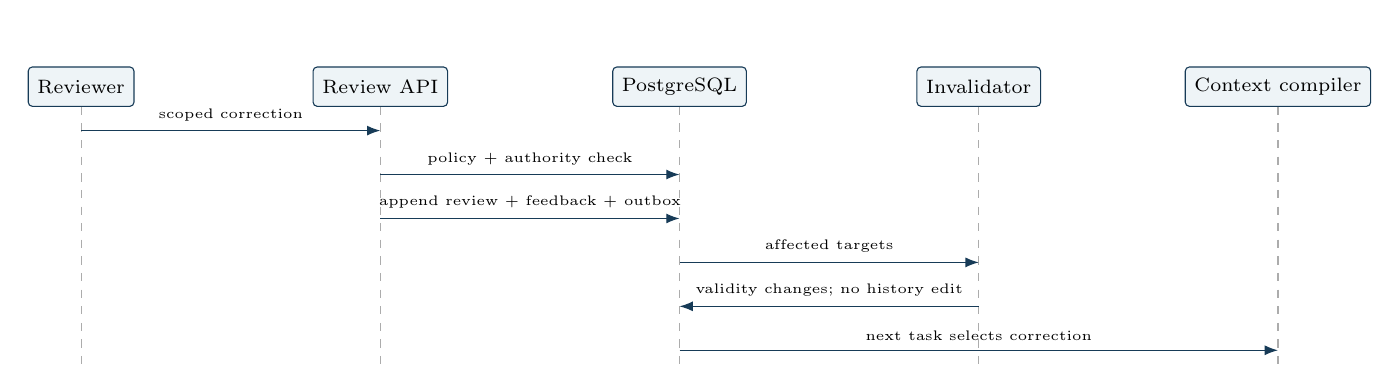
\begin{tikzpicture}[x=0.95cm,y=0.62cm]
\node[seqactor] (u) at (0,0) {Reviewer};
\node[seqactor] (a) at (4,0) {Review API};
\node[seqactor] (d) at (8,0) {PostgreSQL};
\node[seqactor] (i) at (12,0) {Invalidator};
\node[seqactor] (c) at (16,0) {Context compiler};
\foreach \n in {u,a,d,i,c}{\draw[seqlife] (\n.south) -- ++(0,-5.6);}
\draw[seqmsg] (0,-0.9)--node[above,font=\tiny]{scoped correction}(4,-0.9);
\draw[seqmsg] (4,-1.8)--node[above,font=\tiny]{policy + authority check}(8,-1.8);
\draw[seqmsg] (4,-2.7)--node[above,font=\tiny]{append review + feedback + outbox}(8,-2.7);
\draw[seqmsg] (8,-3.6)--node[above,font=\tiny]{affected targets}(12,-3.6);
\draw[seqmsg] (12,-4.5)--node[above,font=\tiny]{validity changes; no history edit}(8,-4.5);
\draw[seqmsg] (8,-5.4)--node[above,font=\tiny]{next task selects correction}(16,-5.4);
\end{tikzpicture}
\caption{Human review creates governed feedback while preserving the original artifact.}
\end{figure}

\begin{figure}[H]
\centering
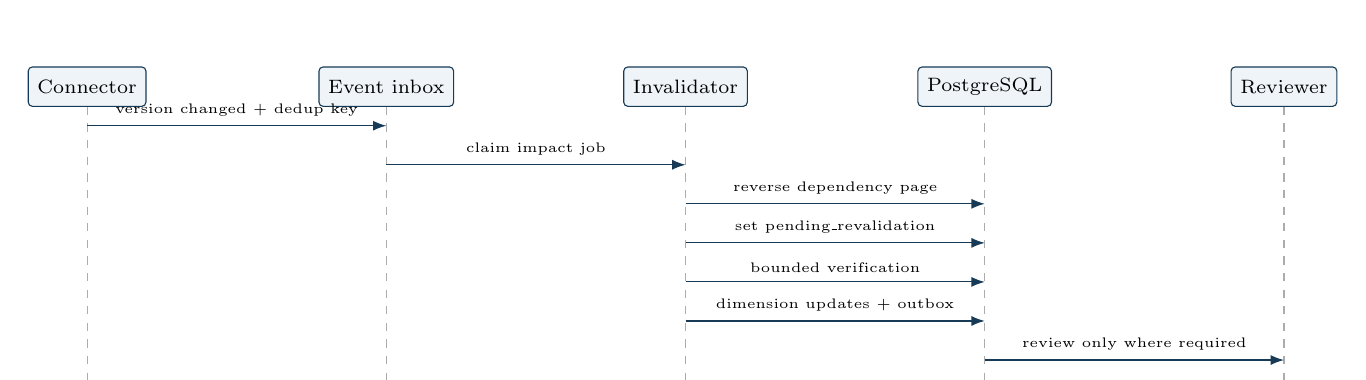
\begin{tikzpicture}[x=0.95cm,y=0.62cm]
\node[seqactor] (s) at (0,0) {Connector};
\node[seqactor] (e) at (4,0) {Event inbox};
\node[seqactor] (i) at (8,0) {Invalidator};
\node[seqactor] (d) at (12,0) {PostgreSQL};
\node[seqactor] (r) at (16,0) {Reviewer};
\foreach \n in {s,e,i,d,r}{\draw[seqlife] (\n.south) -- ++(0,-5.8);}
\draw[seqmsg] (0,-0.8)--node[above,font=\tiny]{version changed + dedup key}(4,-0.8);
\draw[seqmsg] (4,-1.6)--node[above,font=\tiny]{claim impact job}(8,-1.6);
\draw[seqmsg] (8,-2.4)--node[above,font=\tiny]{reverse dependency page}(12,-2.4);
\draw[seqmsg] (8,-3.2)--node[above,font=\tiny]{set pending\_revalidation}(12,-3.2);
\draw[seqmsg] (8,-4.0)--node[above,font=\tiny]{bounded verification}(12,-4.0);
\draw[seqmsg] (8,-4.8)--node[above,font=\tiny]{dimension updates + outbox}(12,-4.8);
\draw[seqmsg] (12,-5.6)--node[above,font=\tiny]{review only where required}(16,-5.6);
\end{tikzpicture}
\caption{Source-change invalidation is deduplicated, paged, bounded, and dimension-specific.}
\end{figure}

\subsection{Replay Sequence}

\begin{figure}[H]
\centering
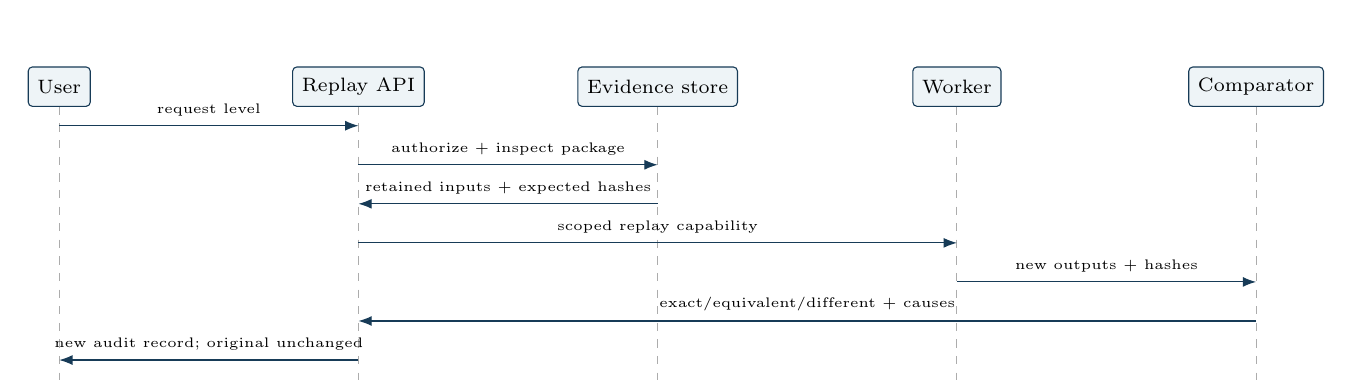
\begin{tikzpicture}[x=0.95cm,y=0.62cm]
\node[seqactor] (u) at (0,0) {User};
\node[seqactor] (a) at (4,0) {Replay API};
\node[seqactor] (d) at (8,0) {Evidence store};
\node[seqactor] (w) at (12,0) {Worker};
\node[seqactor] (v) at (16,0) {Comparator};
\foreach \n in {u,a,d,w,v}{\draw[seqlife] (\n.south) -- ++(0,-5.8);}
\draw[seqmsg] (0,-0.8)--node[above,font=\tiny]{request level}(4,-0.8);
\draw[seqmsg] (4,-1.6)--node[above,font=\tiny]{authorize + inspect package}(8,-1.6);
\draw[seqmsg] (8,-2.4)--node[above,font=\tiny]{retained inputs + expected hashes}(4,-2.4);
\draw[seqmsg] (4,-3.2)--node[above,font=\tiny]{scoped replay capability}(12,-3.2);
\draw[seqmsg] (12,-4.0)--node[above,font=\tiny]{new outputs + hashes}(16,-4.0);
\draw[seqmsg] (16,-4.8)--node[above,font=\tiny]{exact/equivalent/different + causes}(4,-4.8);
\draw[seqmsg] (4,-5.6)--node[above,font=\tiny]{new audit record; original unchanged}(0,-5.6);
\end{tikzpicture}
\caption{Replay creates new evidence and a comparison; it never rewrites the original run.}
\end{figure}

\end{document}
